%!TEX spellcheck
%%%%%%%%%%%%%%%%%%%%%%%%%%%%%%%%%%%%%%%%%
% Beamer Presentation
% LaTeX Template
% Version 2.0 (March 8, 2022)
%
% This template originates from:
% https://www.LaTeXTemplates.com
%
% Author:
% Vel (vel@latextemplates.com)
%
% License:
% CC BY-NC-SA 4.0 (https://creativecommons.org/licenses/by-nc-sa/4.0/)
%
%%%%%%%%%%%%%%%%%%%%%%%%%%%%%%%%%%%%%%%%%

%----------------------------------------------------------------------------------------
%	PACKAGES AND OTHER DOCUMENT CONFIGURATIONS
%----------------------------------------------------------------------------------------

\documentclass[
	11pt, % Set the default font size, options include: 8pt, 9pt, 10pt, 11pt, 12pt, 14pt, 17pt, 20pt
	%t, % Uncomment to vertically align all slide content to the top of the slide, rather than the default centered
	%aspectratio=169, % Uncomment to set the aspect ratio to a 16:9 ratio which matches the aspect ratio of 1080p and 4K screens and projectors
	% handout,
]{beamer}

\graphicspath{{Images/}{./}} % Specifies where to look for included images (trailing slash required)

\usepackage{booktabs} % Allows the use of \toprule, \midrule and \bottomrule for better rules in tables

%----------------------------------------------------------------------------------------
%	SELECT LAYOUT THEME
%----------------------------------------------------------------------------------------

% Beamer comes with a number of default layout themes which change the colors and layouts of slides. Below is a list of all themes available, uncomment each in turn to see what they look like.

%\usetheme{default}
%\usetheme{AnnArbor}
%\usetheme{Antibes}
%\usetheme{Bergen}
%\usetheme{Berkeley}
%\usetheme{Berlin}
%\usetheme{Boadilla}
%\usetheme{CambridgeUS}
%\usetheme{Copenhagen}
%\usetheme{Darmstadt}
%\usetheme{Dresden}
%\usetheme{Frankfurt}
%\usetheme{Goettingen}
%\usetheme{Hannover}
%\usetheme{Ilmenau}
%\usetheme{JuanLesPins}
%\usetheme{Luebeck}
\usetheme{Madrid}
%\usetheme{Malmoe}
%\usetheme{Marburg}
%\usetheme{Montpellier}
%\usetheme{PaloAlto}
%\usetheme{Pittsburgh}
%\usetheme{Rochester}
%\usetheme{Singapore}
%\usetheme{Szeged}
%\usetheme{Warsaw}

%----------------------------------------------------------------------------------------
%	SELECT COLOR THEME
%----------------------------------------------------------------------------------------

% Beamer comes with a number of color themes that can be applied to any layout theme to change its colors. Uncomment each of these in turn to see how they change the colors of your selected layout theme.

%\usecolortheme{albatross}
%\usecolortheme{beaver}
%\usecolortheme{beetle}
%\usecolortheme{crane}
%\usecolortheme{dolphin}
%\usecolortheme{dove}
%\usecolortheme{fly}
%\usecolortheme{lily}
%\usecolortheme{monarca}
%\usecolortheme{seagull}
%\usecolortheme{seahorse}
%\usecolortheme{spruce}
%\usecolortheme{whale}
%\usecolortheme{wolverine}

%----------------------------------------------------------------------------------------
%	SELECT FONT THEME & FONTS
%----------------------------------------------------------------------------------------

% Beamer comes with several font themes to easily change the fonts used in various parts of the presentation. Review the comments beside each one to decide if you would like to use it. Note that additional options can be specified for several of these font themes, consult the beamer documentation for more information.

\usefonttheme{default} % Typeset using the default sans serif font
%\usefonttheme{serif} % Typeset using the default serif font (make sure a sans font isn't being set as the default font if you use this option!)
%\usefonttheme{structurebold} % Typeset important structure text (titles, headlines, footlines, sidebar, etc) in bold
%\usefonttheme{structureitalicserif} % Typeset important structure text (titles, headlines, footlines, sidebar, etc) in italic serif
%\usefonttheme{structuresmallcapsserif} % Typeset important structure text (titles, headlines, footlines, sidebar, etc) in small caps serif

%------------------------------------------------

%\usepackage{mathptmx} % Use the Times font for serif text
\usepackage{palatino} % Use the Palatino font for serif text
\usepackage{hyperref}
%\usepackage{helvet} % Use the Helvetica font for sans serif text
\usepackage[default]{opensans} % Use the Open Sans font for sans serif text
%\usepackage[default]{FiraSans} % Use the Fira Sans font for sans serif text
%\usepackage[default]{lato} % Use the Lato font for sans serif text
\usepackage{ctex}
\usepackage{siunitx}
\usepackage{tabularx}
\usepackage{umoline}
\usepackage{fourier}
%----------------------------------------------------------------------------------------
%	SELECT INNER THEME
%----------------------------------------------------------------------------------------

% Inner themes change the styling of internal slide elements, for example: bullet points, blocks, bibliography entries, title pages, theorems, etc. Uncomment each theme in turn to see what changes it makes to your presentation.

%\useinnertheme{default}
\useinnertheme{circles}
%\useinnertheme{rectangles}
%\useinnertheme{rounded}
%\useinnertheme{inmargin}

%----------------------------------------------------------------------------------------
%	SELECT OUTER THEME
%----------------------------------------------------------------------------------------

% Outer themes change the overall layout of slides, such as: header and footer lines, sidebars and slide titles. Uncomment each theme in turn to see what changes it makes to your presentation.

%\useoutertheme{default}
%\useoutertheme{infolines}
%\useoutertheme{miniframes}
%\useoutertheme{smoothbars}
%\useoutertheme{sidebar}
%\useoutertheme{split}
%\useoutertheme{shadow}
%\useoutertheme{tree}
%\useoutertheme{smoothtree}

%\setbeamertemplate{footline} % Uncomment this line to remove the footer line in all slides
%\setbeamertemplate{footline}[page number] % Uncomment this line to replace the footer line in all slides with a simple slide count

%\setbeamertemplate{navigation symbols}{} % Uncomment this line to remove the navigation symbols from the bottom of all slides

%----------------------------------------------------------------------------------------
%	PRESENTATION INFORMATION
%----------------------------------------------------------------------------------------

\title[Geometry]{Geometry} % The short title in the optional parameter appears at the bottom of every slide, the full title in the main parameter is only on the title page

\subtitle{几何} % Presentation subtitle, remove this command if a subtitle isn't required

\author[张凡]{张凡} % Presenter name(s), the optional parameter can contain a shortened version to appear on the bottom of every slide, while the main parameter will appear on the title slide

\institute[XDF]{新东方国际教育 \\ \smallskip \textit{zhangfan@xdf.cn}} % Your institution, the optional parameter can be used for the institution shorthand and will appear on the bottom of every slide after author names, while the required parameter is used on the title slide and can include your email address or additional information on separate lines

\date[\today]{GRE 冲分班数学 \\ \today} % Presentation date or conference/meeting name, the optional parameter can contain a shortened version to appear on the bottom of every slide, while the required parameter value is output to the title slide

%----------------------------------------------------------------------------------------


%----------------------------------------------------------------------------------------
%	Section Slide
%----------------------------------------------------------------------------------------
\AtBeginSection[]{
  \begin{frame}
  \vfill
  \centering
  \begin{beamercolorbox}[sep=8pt,center,shadow=true,rounded=true]{title}
    \usebeamerfont{title}\insertsectionhead\par%
  \end{beamercolorbox}
  \vfill
  \end{frame}

%----------------------------------------------------------------------------------------
%	TABLE OF CONTENTS SLIDE OF THE CURRENT SECTION
%----------------------------------------------------------------------------------------
	\begin{frame}
		\frametitle{Presentation Overview for \secname} % Slide title, remove this command for no title
		\tableofcontents[currentsection, hideothersubsections, sectionstyle=show/show]
	\end{frame}
  }

%----------------------------------------------------------------------------------------

\AtBeginSubsection[]{
  \begin{frame}
  \vfill
  \centering
    \usebeamerfont{title}\insertsubsectionhead\par%
  \vfill
  \end{frame}
}
%----------------------------------------------------------------------------------------


\begin{document}

%----------------------------------------------------------------------------------------
%	TITLE SLIDE
%----------------------------------------------------------------------------------------

\begin{frame}
	\titlepage % Output the title slide, automatically created using the text entered in the PRESENTATION INFORMATION block above
\end{frame}



%----------------------------------------------------------------------------------------
%	PRESENTATION BODY SLIDES
%----------------------------------------------------------------------------------------
\begin{frame}
	\frametitle{To Begin With} % Slide title, remove this command for no title

	\begin{block}{QR Mathematical Convention 3}
		All figures are assumed to lie in a plane unless otherwise indicated.
	\end{block}

		\begin{block}{QR Mathematical Convention 4}
		Geometric figures are not necessarily drawn to scale.
	\end{block}
	\begin{example}
		\begin{itemize}
			\item \alert{Can not} assume  that quantities such as lengths and  are as they appear in a figure
			\item \alert{Can not} assume  that angle measures such as lengths and  are as they appear in a figure 
			\item \alert{Can} assume all geometric objects are in the relative positions shown.
		\end{itemize}
	\end{example}
\end{frame}

%------------------------------------------------

\begin{frame}
	\frametitle{Rely on Your Geometric Reasoning, not Estimating or Comparing Quantities By Eyesight} % Slide title, remove this command for no title
	\framesubtitle{用几何推理做题!}
	\begin{columns}[t] 
		\begin{column}{0.4\textwidth} % Left column width
		Which of the following statements \alert{Must Be} right?
			\begin{figure}
				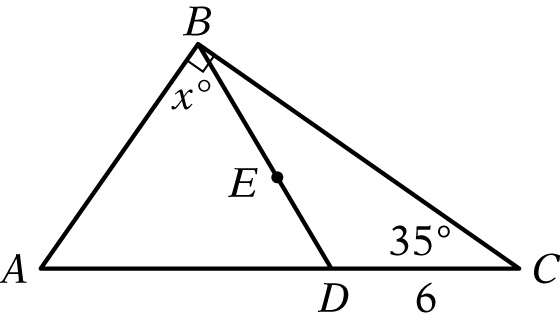
\includegraphics[width=\linewidth]{Not_Scale.jpg}
			\end{figure}
		\end{column}

	\begin{column}{0.6\textwidth} % Right column width
	\begin{enumerate}
		\item Points $A$, $D$, and $C$ are distinct. Point $D$ lies between points $A$ and $C$, and the line containing them is straight.
		\item The length of line segment $AD$ is less than the length of line segment $AC$.
		\item $ABC,\ ABD,\ $ and $DBC$ are triangles.
		\item Point $E$ lies on line segment $BD$.
		\item Angle $ABC$ is a right angle, as indicated by the small square symbol at point $B$.
		\item The length of line segment $DC$ is 6, and the measure of angle $C$ is 35 degrees.
		\item The measure of angle $ABD$ is x degrees, and $x<90$.
	\end{enumerate}
	\end{column}
	\end{columns}
\end{frame}

%------------------------------------------------

\begin{frame}
	\frametitle{Rely on Your Geometric Reasoning, not Estimating or Comparing Quantities By Eyesight} % Slide title, remove this command for no title
	\framesubtitle{用几何推理做题!}
	\begin{columns}[t] 
		\begin{column}{0.4\textwidth} % Left column width
		Which of the following statements \alert{Must Be} right?
			\begin{figure}
				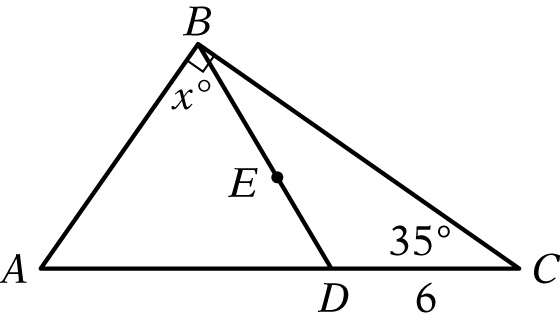
\includegraphics[width=\linewidth]{Not_Scale.jpg}
			\end{figure}
				Answer: \textbf{\alert{They all must be right!}}
		\end{column}

	\begin{column}{0.6\textwidth} % Right column width
	\begin{enumerate}
		\item Points $A$, $D$, and $C$ are distinct. Point D lies between points $A$ and $C$, and the line containing them is straight.
		\item The length of line segment $AD$ is less than the length of line segment $AC$.
		\item $ABC,\ ABD,\ $ and $DBC$ are triangles.
		\item Point $E$ lies on line segment $BD$.
		\item Angle $ABC$ is a right angle, as indicated by the small square symbol at point $B$.
		\item The length of line segment $DC$ is 6, and the measure of angle $C$ is 35 degrees.
		\item The measure of angle $ABD$ is x degrees, and $x<90$.
	\end{enumerate}
	\end{column}
	\end{columns}
\end{frame}

%------------------------------------------------

\begin{frame}
	\frametitle{Rely on Your Geometric Reasoning, not Estimating or Comparing Quantities By eyesight} % Slide title, remove this command for no title
	\framesubtitle{用几何推理做题!}
	\begin{columns}[t] 
		\begin{column}{0.4\textwidth} % Left column width
		Which of the following statements \alert{Must Be} right?
			\begin{figure}
				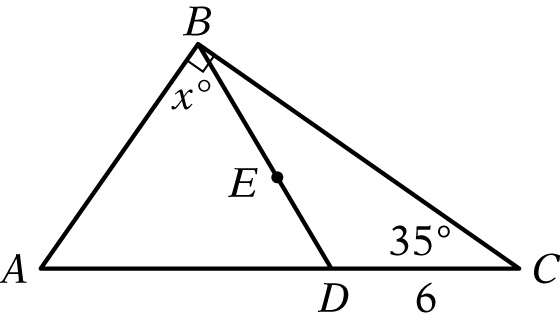
\includegraphics[width=\linewidth]{Not_Scale.jpg}
			\end{figure}
		\end{column}

	\begin{column}{0.6\textwidth} % Right column width
	\begin{enumerate}
		\item The length of line segment $AD$ is greater than the length of line segment $DC$.
		\item The measures of angles $BAD$ and $BDA$ are equal.
		\item The measure of angle is less than x degrees.
		\item The area of triangle $ABD$ is greater than the area of triangle $DBC$.
	\end{enumerate}
	\pause
	Answer: \textbf{\alert{They are all not necessarily right!}}
	\end{column}
	\end{columns}
\end{frame}

%------------------------------------------------

% vertices raddii plura

%------------------------------------------------

\section{Lines and Angles}

%------------------------------------------------

\subsection{Lines}

%------------------------------------------------

\begin{frame}
	\frametitle{Congruent line segments} % Slide title, remove this command for no title
	\framesubtitle{全等线段}
	\framesubtitle{用几何推理做题!}
		\begin{figure}
			\includegraphics[width=\linewidth]{Lines.jpg}
			\caption{$BC$ and $CD$ are congruent line segments.}
		\end{figure}

		\begin{definition}
		Line segments that have equal lengths are called \alert{congruent line segments} .
		\end{definition}
\end{frame}

%------------------------------------------------

\begin{frame}
	\frametitle{Math Vocab!} % Slide title, remove this command for no title
	\framesubtitle{专业名词记忆时间!}
	
	{\Huge congruent}\\
	{\LARGE /kənˈɡro͞oənt,ˈkäNGɡro͞oənt/\\
		\bigskip\bigskip
	(of figures) identical in form; coinciding exactly when superimposed. \\ 
	全等:相同,叠加的时候完全重合}

\end{frame}

%------------------------------------------------



%------------------------------------------------

\subsection{Angles}

%------------------------------------------------

\begin{frame}
	\frametitle{Opposite Angles} % Slide title, remove this command for no title
	\framesubtitle{对角相等}
	\begin{columns}[t] 
		\begin{column}{0.4\textwidth} % Left column width
			\begin{figure}
				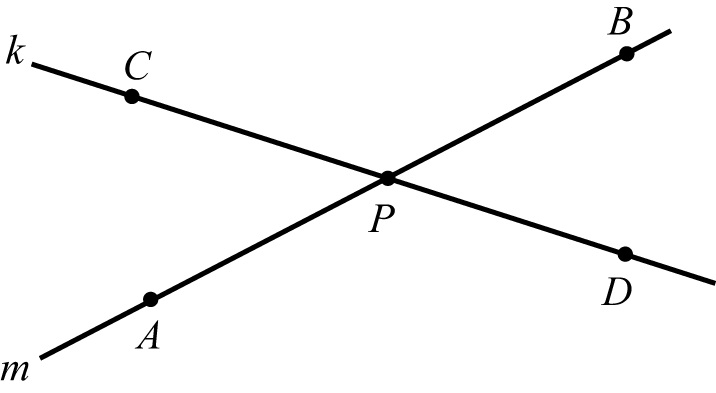
\includegraphics[width=\linewidth]{Angles.jpg}
				\caption{$\angle APC$ and $\angle BPD$ are opposite angles; So are  $\angle CPB$ and $\angle DPA$.}
			\end{figure}
		\end{column}

	\begin{column}{0.6\textwidth} % Right column width
		\begin{definition}
		Opposite angles have equal measure, and angles that have equal measure are called congruent angles. Hence, \alert{opposite angles are congruent}.
		\end{definition}
	\end{column}
	\end{columns}
\end{frame}

%------------------------------------------------

\begin{frame}
	\frametitle{Acute,Right, Obtuse Angles} % Slide title, remove this command for no title
	\framesubtitle{锐角\ 直角\ 钝角}

		\begin{figure}
			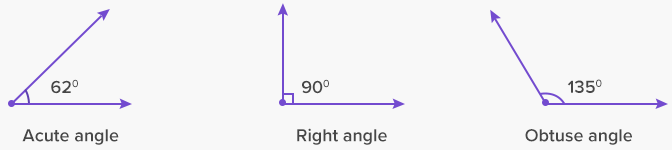
\includegraphics[width=\linewidth]{Acute_Right_Obtuse.png}
			\caption{$BC$ and $CD$ are congruent line segments.}
		\end{figure}

		\begin{definition}
		\begin{itemize}
			\item An angle with measure less than 90° is called an \alert{acute angle}.
			\item An angle with a measure of 90° is called a \alert{right angle}.
			\item an angle with measure between 90° and 180° is called an \alert{obtuse angle}.
		\end{itemize}
		\end{definition}
\end{frame}

%------------------------------------------------

\subsection{Parallel Lines}

%------------------------------------------------

\begin{frame}
	\frametitle{Parallel Lines} % Slide title, remove this command for no title
	\framesubtitle{平行线同位角相等,内错角之和为180度}
		\begin{figure}
			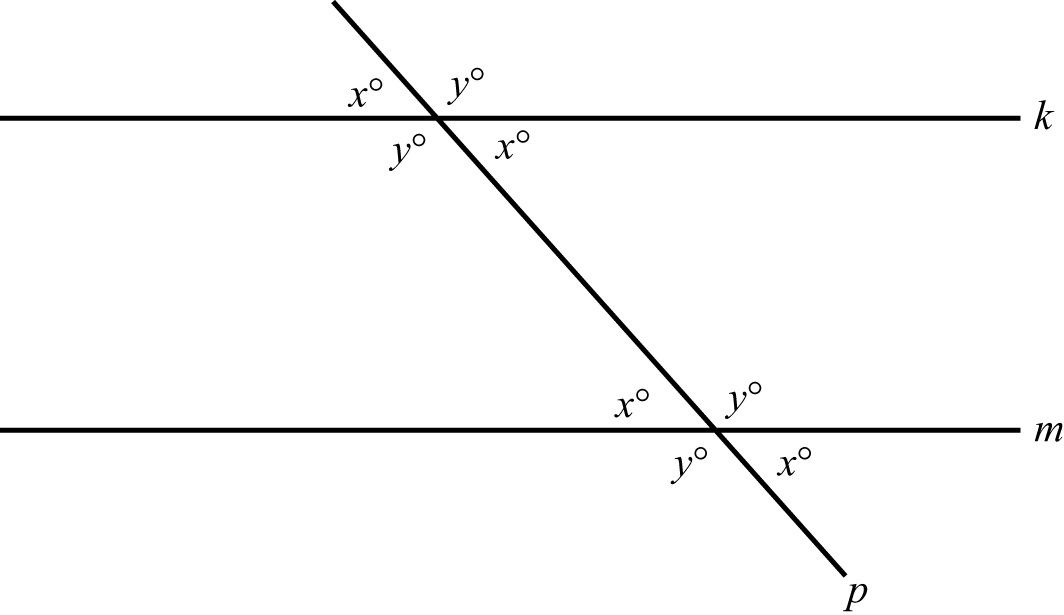
\includegraphics[width=0.9\linewidth]{Parallel_Lines.jpg}
			\caption{$k \parallel m$}
		\end{figure}
\end{frame}

%------------------------------------------------

\section{Triangles}

%------------------------------------------------

\subsection{Equilateral Triangles}

%------------------------------------------------

\begin{frame}
	\frametitle{Math Vocab!} % Slide title, remove this command for no title
	\framesubtitle{专业名词记忆时间!}
	
	{\Huge Equilateral}\\
	{\LARGE /ˌēkwəˈladərəl,ˌekwəˈladərəl/\\
		\bigskip\bigskip
	(of figures) having all its sides of the same length.. \\ 
	等边:所有边长相等}

\end{frame}

%------------------------------------------------

\begin{frame}
	\frametitle{Equilateral Triangles} % Slide title, remove this command for no title
	\framesubtitle{等边三角形:内角均为60度}

		\begin{figure}
			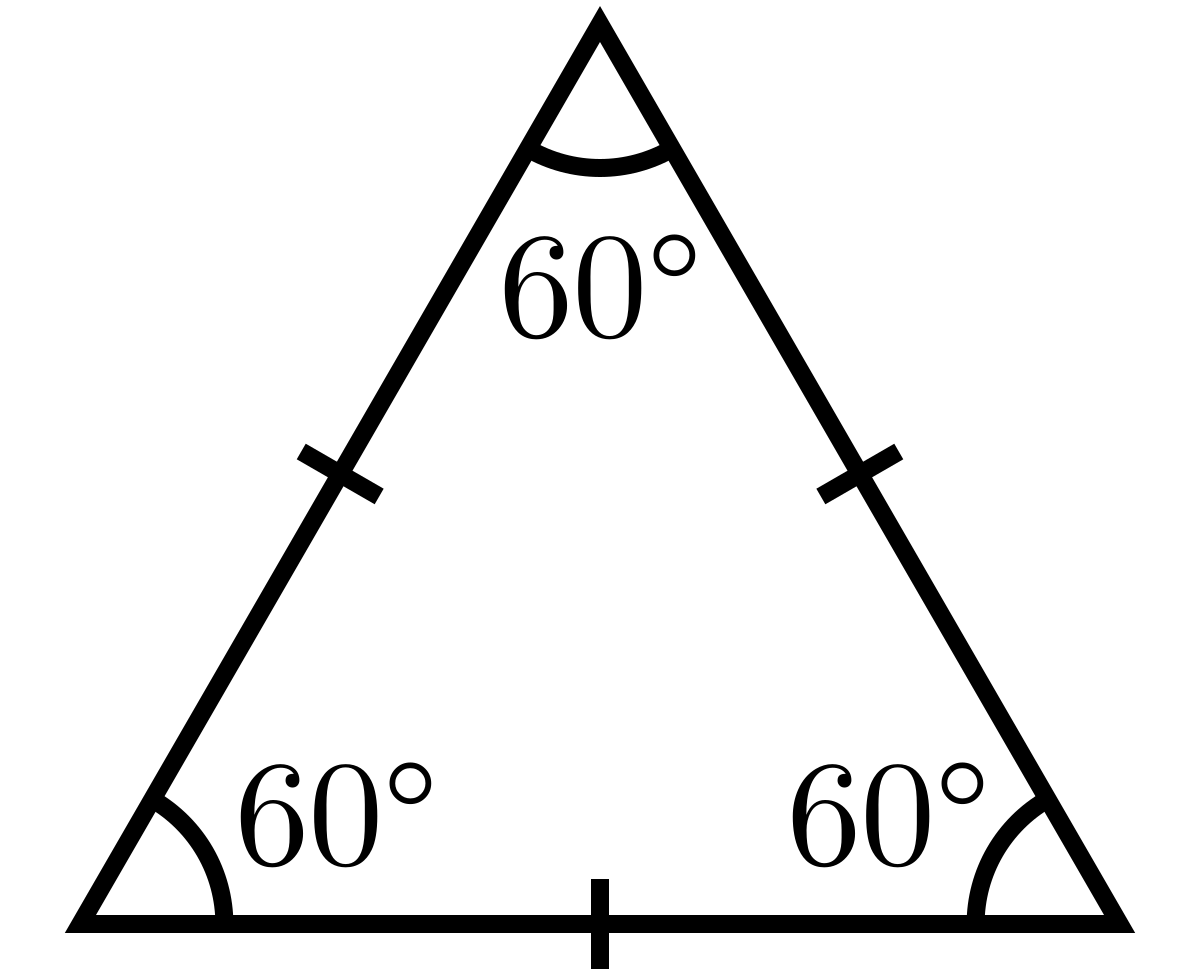
\includegraphics[width=0.6\linewidth]{Triangle.Equilateral.svg.png}
			\caption{The measures of the three interior angles of  a equilateral triangle are
equal, and each measure is 60°.}
		\end{figure}
\end{frame}

%------------------------------------------------


\begin{frame}
	\frametitle{A Real QR Problem!}
	\framesubtitle{自己画图!}
	\begin{figure}
		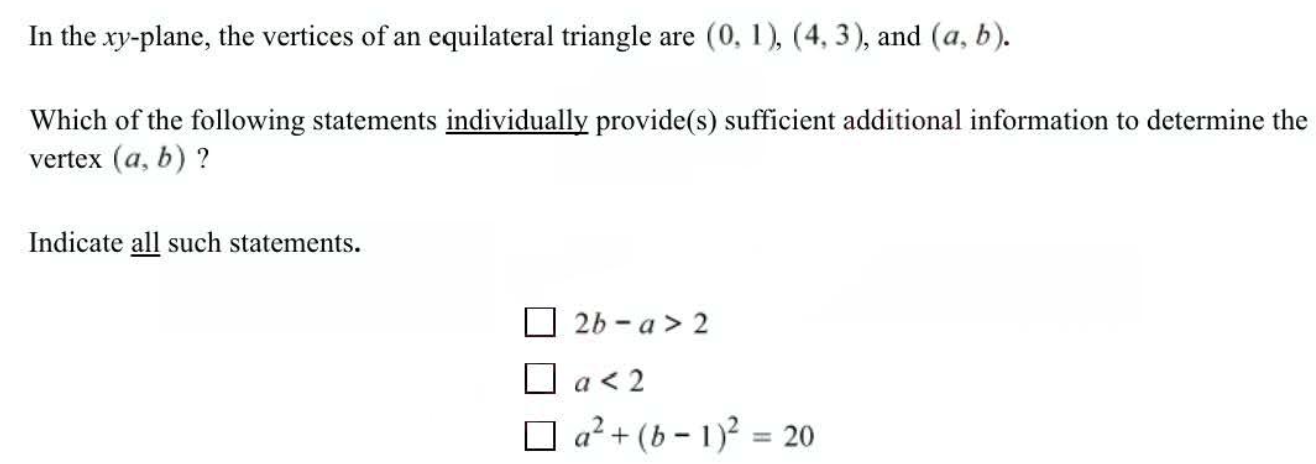
\includegraphics[width=\linewidth]{Equilateral_Triangles_Example_Question1.png}
		\caption{2-Sec2-13}
	\end{figure}

\end{frame}

%------------------------------------------------


\begin{frame}
	\frametitle{Answer}
	\framesubtitle{自己画图!}
	\pause
	\begin{figure}
		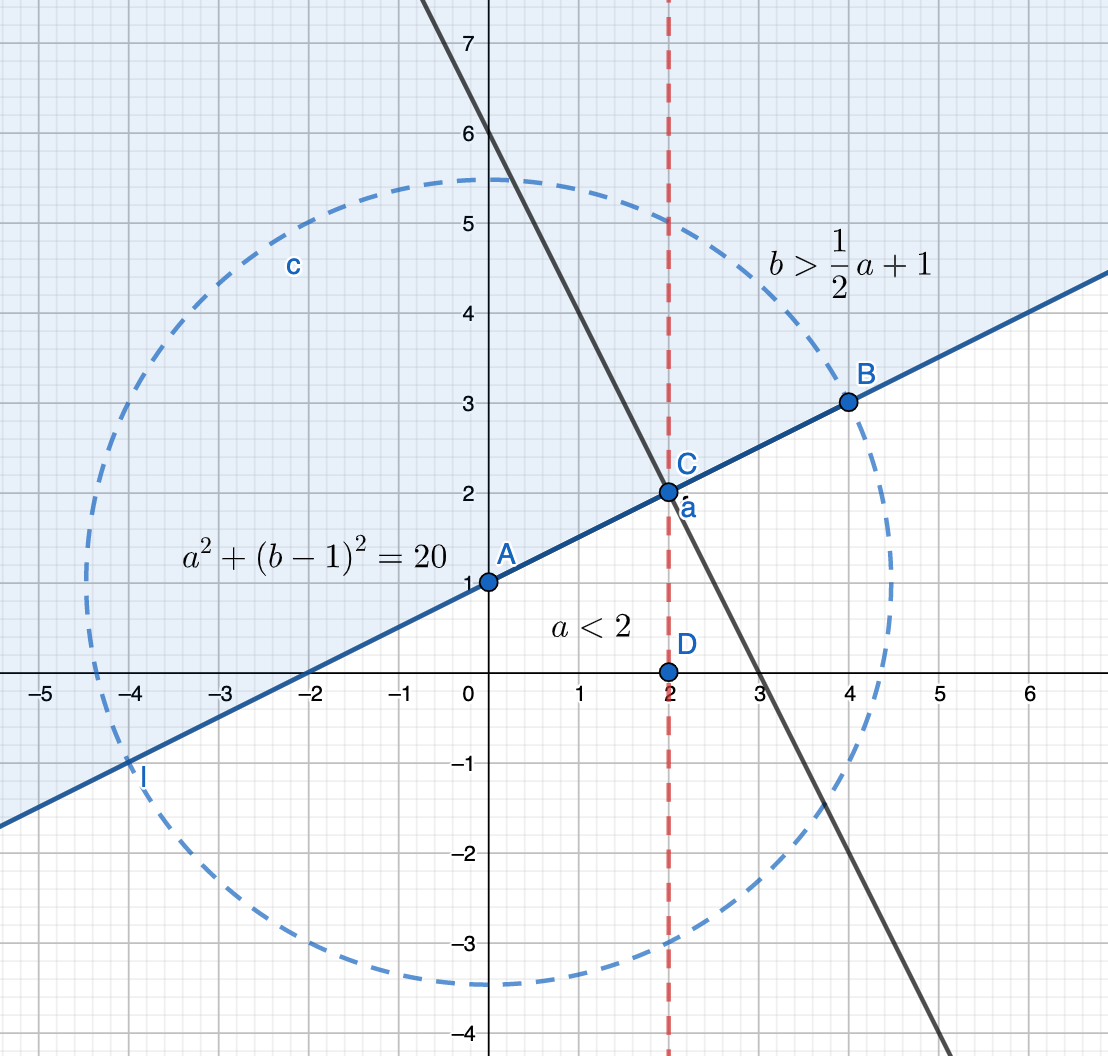
\includegraphics[width=0.5\linewidth]{Equilateral_Triangles_Example_Question1_1.png}
	\end{figure}
	\pause
\bigskip
Answer \textbf{AB} $b =  \frac{1}{2} a + 1 $       $a<2$
\end{frame}

%------------------------------------------------

\subsection{Isosceles Triangles}

%------------------------------------------------

\begin{frame}
	\frametitle{Math Vocab!} % Slide title, remove this command for no title
	\framesubtitle{专业名词记忆时间!}
	
	{\Huge Isosceles}\\
	{\LARGE /īˈsäsəˌlēz/\\
		\bigskip\bigskip
	(of a triangle) having two sides of equal length. \\ 
	等腰三角形:两边长相等}

\end{frame}

%------------------------------------------------

\begin{frame}
	\frametitle{Isosceles Triangles} % Slide title, remove this command for no title
	\framesubtitle{等腰三角形:内角均为60度}



	\begin{columns}[t] 

		\begin{column}{0.5\textwidth} % Left column width
			\begin{figure}
				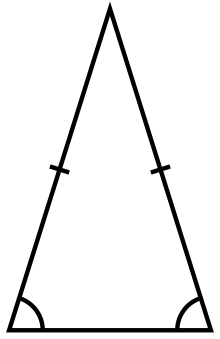
\includegraphics[width=0.5\linewidth]{220px-Triangle.Isosceles.svg.png}
				\caption{Congruent sides suggest congruent angles.}
			\end{figure}		
		\end{column}
		\begin{column}{0.5\textwidth} % Right column width
		\begin{theorem}[两角相等互推两边相等]
			If a triangle has two congruent sides, then the angles opposite
the two congruent sides are congruent. \alert{The converse is also true}.
		\end{theorem}
		\pause
		\begin{theorem}[Law Of Sines\ 正弦定理]
			\begin{equation*}
				\frac{\sin A}{a}=\frac{\sin B}{b}=\frac{\sin C}{c}
			\end{equation*}
		\end{theorem}
		\end{column}
	\end{columns}
\end{frame}

%------------------------------------------------


\begin{frame}
	\frametitle{Have a try!}
	\framesubtitle{}
An isosceles triangle lies on the rectangular coordinate plane, the coordinates of
point A are (0, 0), and the coordinates of point B are (3, 1), point C could lie at one of
6 positions such that (1, 3), (-1, 3), (-3, 1), (-1, -3), (1, -3), (3, -1). How many lengths of
side BC are possible?\\
	\begin{columns}[t] 
		\begin{column}{0.8\textwidth} % Left column width
		\begin{figure}
			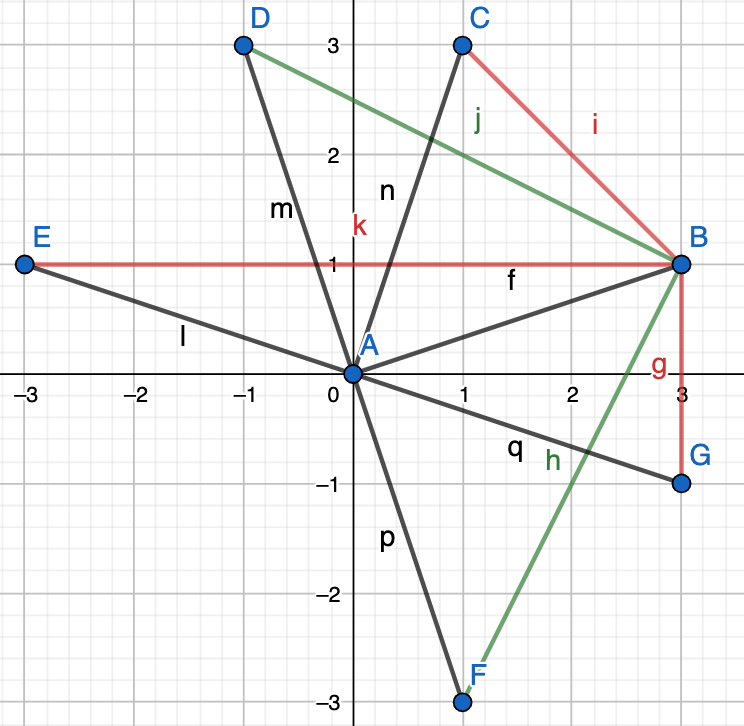
\includegraphics[width=0.5\linewidth]{Isosceles_Example_Question1.png}
			\caption{$BD$ and $BF$ have the same length}
		\end{figure}
		\end{column}
		\begin{column}{0.2\textwidth} % Right column width
		\pause
		\bigskip
		Answer \textbf{5}
		\end{column}
	\end{columns}





\end{frame}

%------------------------------------------------

\subsection{Right Triangles}

%------------------------------------------------

\begin{frame}
	\frametitle{Math Vocab!} % Slide title, remove this command for no title
	\framesubtitle{专业名词记忆时间!}
	
	\begin{columns}[t] 
		\begin{column}{0.7\textwidth} % Left column width
			{\Huge hypotenuse}\\
	{\LARGE /hīˈpätnˌ(y)o͞os/\\
		\bigskip\bigskip
	the longest side of a right triangle, opposite the right angle. \\ 
	斜边:直角三角形直角对边}
	\bigskip\bigskip\bigskip\bigskip

		{\Huge leg}\\{\LARGE 直角边}
		\end{column}
		\begin{column}{0.3\textwidth} % Right column width
					\begin{figure}
				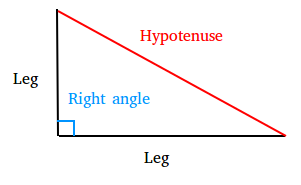
\includegraphics[width=\linewidth]{Hypotenuse.png}
			\end{figure}	
		\end{column}
	\end{columns}
\end{frame}

%------------------------------------------------

\begin{frame}
	\frametitle{The Pythagorean Theorem} % Slide title, remove this command for no title
	\framesubtitle{勾股定理}
	\begin{figure}
		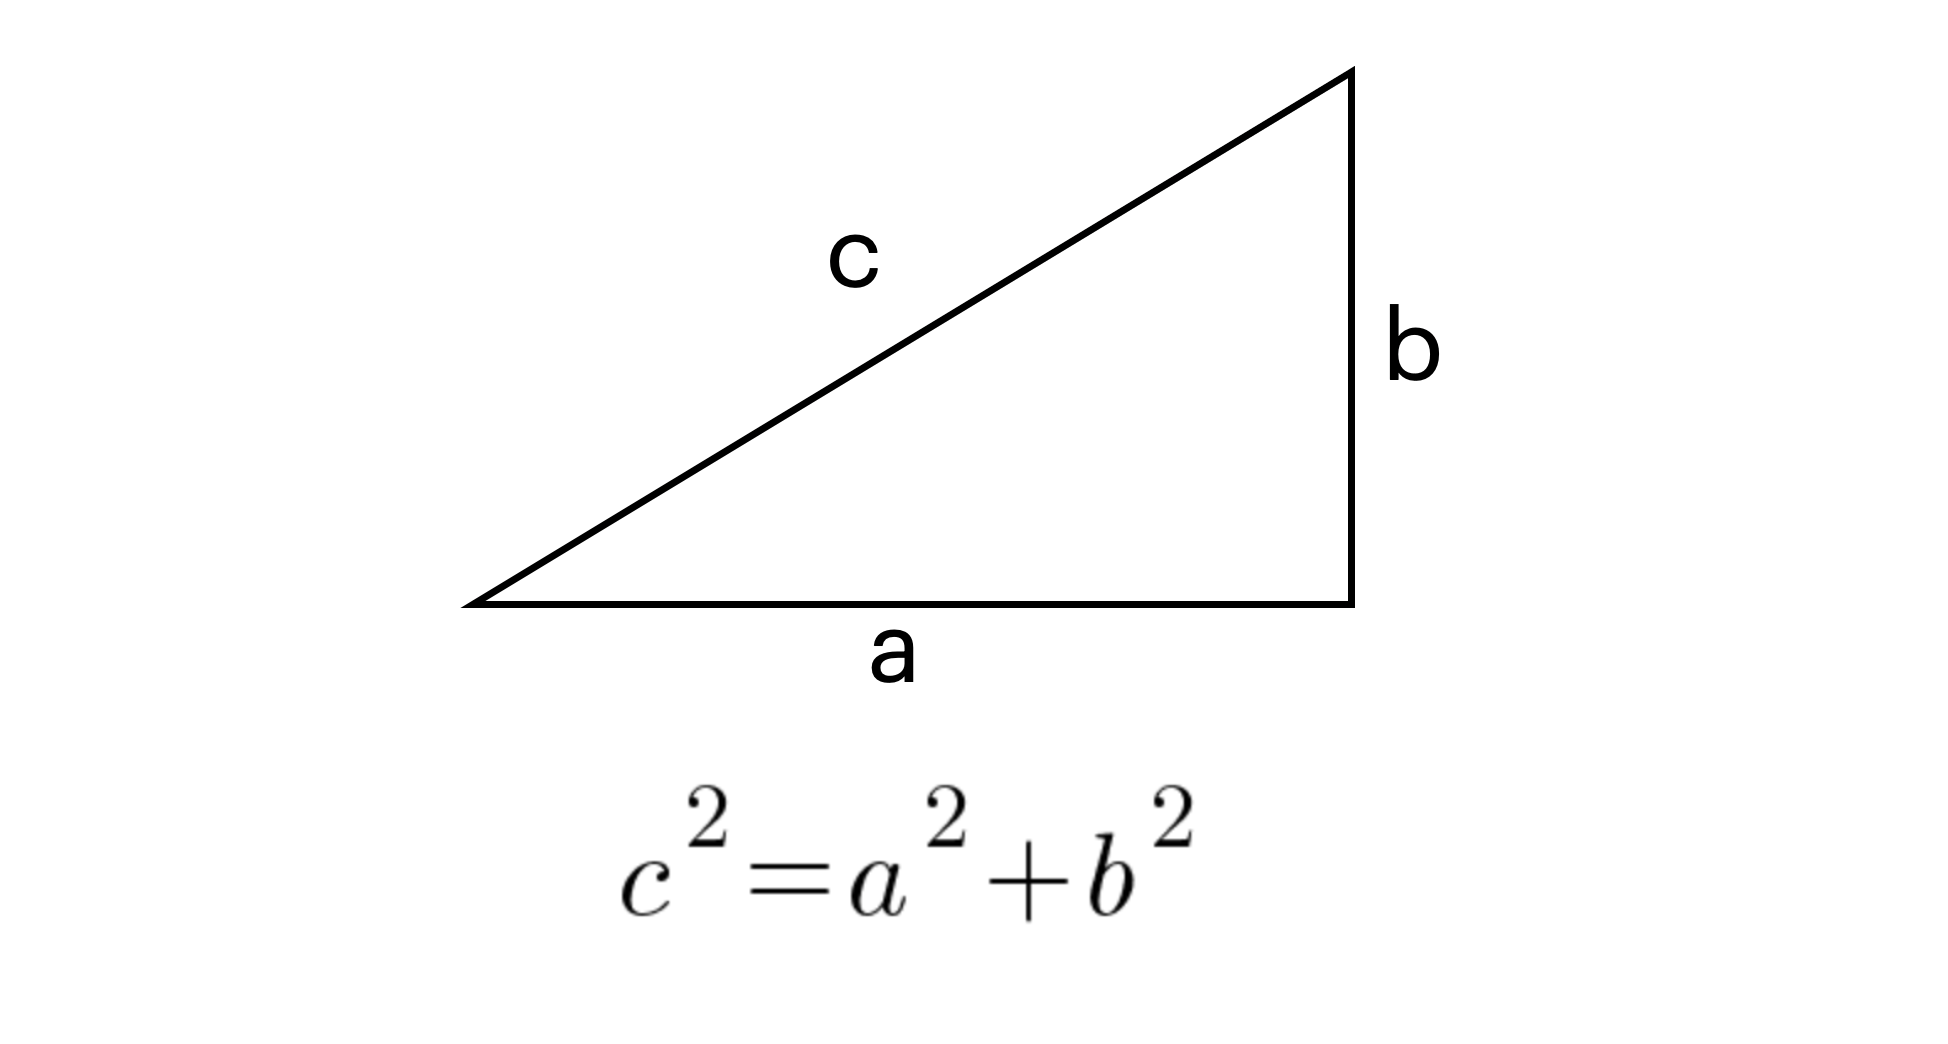
\includegraphics[width=\linewidth]{Pythagorean.png}
	\end{figure}	
\end{frame}

%------------------------------------------------

\begin{frame}
	\frametitle{Math Vocab!} % Slide title, remove this command for no title
	\framesubtitle{专业名词记忆时间!}
	
	{\Huge Pythagorean}\\
	{\LARGE /īˈsäsəˌlēz/\\
		\bigskip\bigskip
	relating to or characteristic of the Greek philosopher Pythagoras or his ideas. \\ 
	毕达哥拉斯}
\end{frame}

%------------------------------------------------

\begin{frame}
	\frametitle{Have a try!}

A ladder 25 feet long is leaning against a wall that is perpendicular to level ground.
The bottom of the ladder is 7 feet from the base of the wall. If the top of the ladder
slips down 4 feet, how many feet will the bottom of the ladder slip?\\

\bigskip
\pause
$\sqrt{(25^2 - (7-4)^2) - (25^2- 7^2)} = 2\sqrt{10}\approx =6.32 feet $\\
\bigskip\pause
Answer \textbf{6.32 Feet} \pause 
\\\alert{QR只能一个空之能填一个数,没有根号输入}
\end{frame}

%------------------------------------------------

\begin{frame}
	\frametitle{A Real QR Problem!}
	\framesubtitle{注意“could be”}
	\begin{figure}
		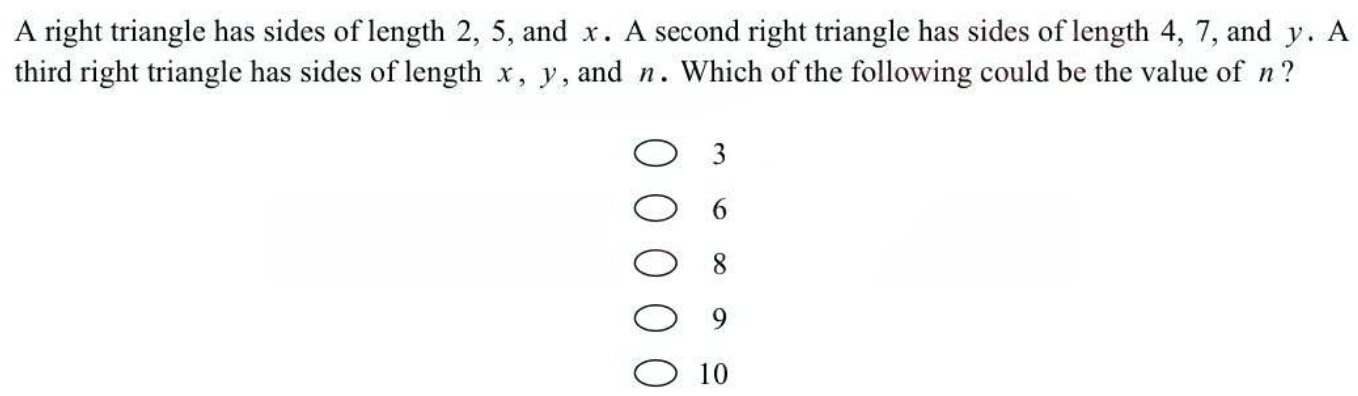
\includegraphics[width=\linewidth]{Pythagorean_Example_Question2.png}
		\caption{8-Sec3-18}
	\end{figure}

\end{frame}

%------------------------------------------------


\begin{frame}
	\frametitle{Answer}
	\pause
	\begin{columns}[t] 
		\begin{column}{0.33\textwidth} % Left column width
			\begin{equation*}
				\begin{aligned}
					&case \ 1:\ x\ is\ hypotenuse\\
					&x^2 = 2^2 + 5^2 = 29\\
					&case \ 2:\ 5\ is\ hypotenuse\\
					&x^2 =  5^2 -2^2 = 21\\	
					&case \ 3:\ y\ is\ hypotenuse\\
					&y^2 =  4^2 + 7^2 = 65\\
					&case \ 4:\ 7\ is\ hypotenuse\\
					&y^2 =   7^2 - 4^2  = 33\\	
				\end{aligned}
			\end{equation*}		
		\end{column}

		\begin{column}{0.33\textwidth} % Left column width
			\begin{equation*}
				\begin{aligned}
					&case \ 5:\ n\ is\ hypotenuse\\
					&n^2 =   x^2 + y^2 \\
					&= 29+65 = 94\ discarded!\\
					&= 29+33 = 62\ discarded!\\	
					&= 21+65 = 86\ discarded!\\
					&= 21+33 = 54\ discarded!\\	
					&case\ 6:\ y\ is\ hypotenuse\\
					&n^2 =   y^2 - x^2 \\
					&= 65 - 29= 36\ B!\\
					&= 33-29 = 4\ Not\ shown!\\	
					&= 65 - 21 = 44\ discarded!\\
					&= 33 - 21 = 12\ discarded!\\	
				\end{aligned}
			\end{equation*}			
		\end{column}

		\begin{column}{0.33\textwidth} % Left column width
			\pause
			Answer \textbf{B } 6
		\end{column}			
	\end{columns}
\end{frame}





%------------------------------------------------

\begin{frame}
	\frametitle{45°-45°-90° Triangle} % Slide title, remove this command for no title
	\framesubtitle{边长比为1:1:$\sqrt{2}$}
	\begin{figure}
		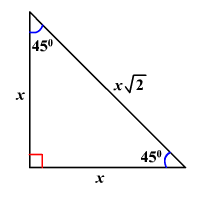
\includegraphics[width=0.5\linewidth]{45-45-90-Triangle.png}
		\caption{\alert{Isosceles Right Triangle}}
	\end{figure}	
\end{frame}

%------------------------------------------------


\begin{frame}
	\frametitle{Have a try!}
	\framesubtitle{}
In the figure above, AB = BC = CD = DE, all triangles are right triangles. If AE = 10,
what is the length of AB?\\

	\begin{columns}[t] 
		\begin{column}{0.4\textwidth} % Left column width
			\begin{figure}
		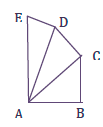
\includegraphics[width=\linewidth]{Right_Triangle_Example_Question2.png}
	\end{figure}	
		\end{column}
		\begin{column}{0.55\textwidth} % Right column width
		\pause
		\begin{equation*}
			\begin{aligned}
				&AE^2= ED^2 + AD^2 \\
				&= ED^2 + (CD^2 + AC^2)\\
				&= ED^2 + (CD^2 + AB^2 + BC^2)\\
				&= 4AB^2 \\
				&= 100\\
				&\therefore AB = \sqrt{25} =5
			\end{aligned}
		\end{equation*}
		\bigskip
		Answer \textbf{5}
		\end{column}
	\end{columns}


\end{frame}

%------------------------------------------------

\begin{frame}
	\frametitle{30°-60°-90° Triangle} % Slide title, remove this command for no title
	\framesubtitle{边长比为1:$\sqrt{3}$:2}
	\begin{figure}
		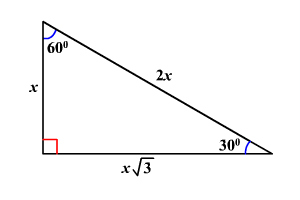
\includegraphics[width=0.5\linewidth]{30_60_90_triangle.png}
	\end{figure}	
\end{frame}


%------------------------------------------------


\begin{frame}
	\frametitle{A Real QR Problem!}
	\framesubtitle{}
	\begin{figure}
		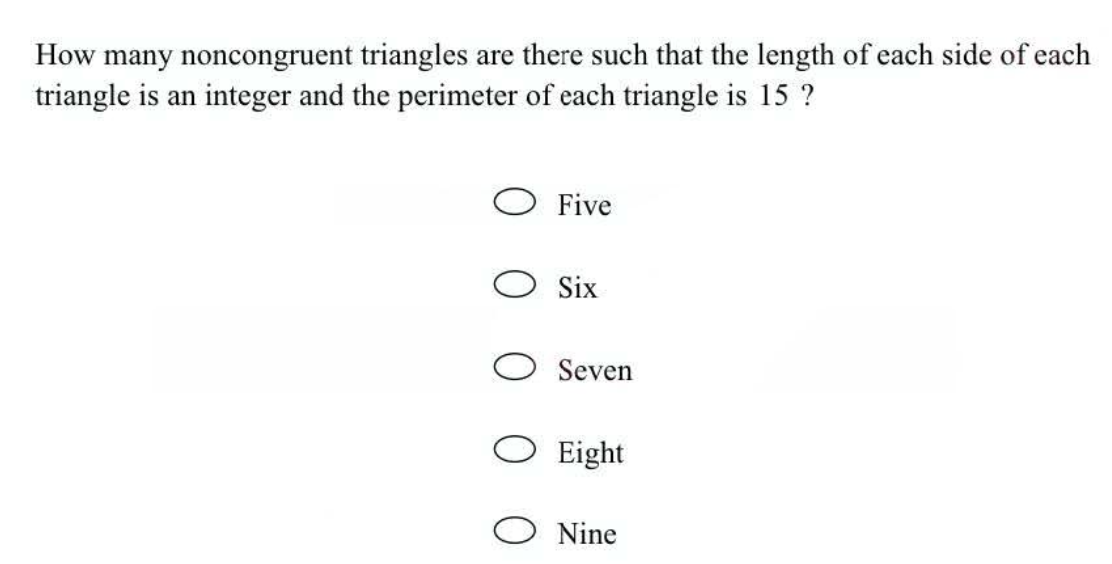
\includegraphics[width=\linewidth]{Triangle_Inequalities_Example_Question1.png}
		\caption{8-Sec2-12}
	\end{figure}

\end{frame}

%------------------------------------------------


\begin{frame}
	\frametitle{The Pythagorean Inequality For The Obtuse Triangles} % Slide title, remove this command for no title
	\framesubtitle{钝角三角形长边平方大于两短边平方和}
	\begin{theorem}
	In an obtuse triangle, the square of the longest side will be greater than adding the two squares of the shorter sides.
	\end{theorem}
	\begin{columns}[t] 
		\begin{column}{0.3\textwidth} % Left column width
			\begin{equation*}
				\begin{aligned}
					&BC^2 = DC^2 + DB^2 \\
					& = (AC^2 - AD^2) + \\
					& AD^2 + AB^2 + 2AD\cdot AB\\
					&>AC^2 + AB^2 \ Q.E.D.
				\end{aligned}
			\end{equation*}					
		\end{column}
		\begin{column}{0.7\textwidth} % Right column width
			\begin{figure}
				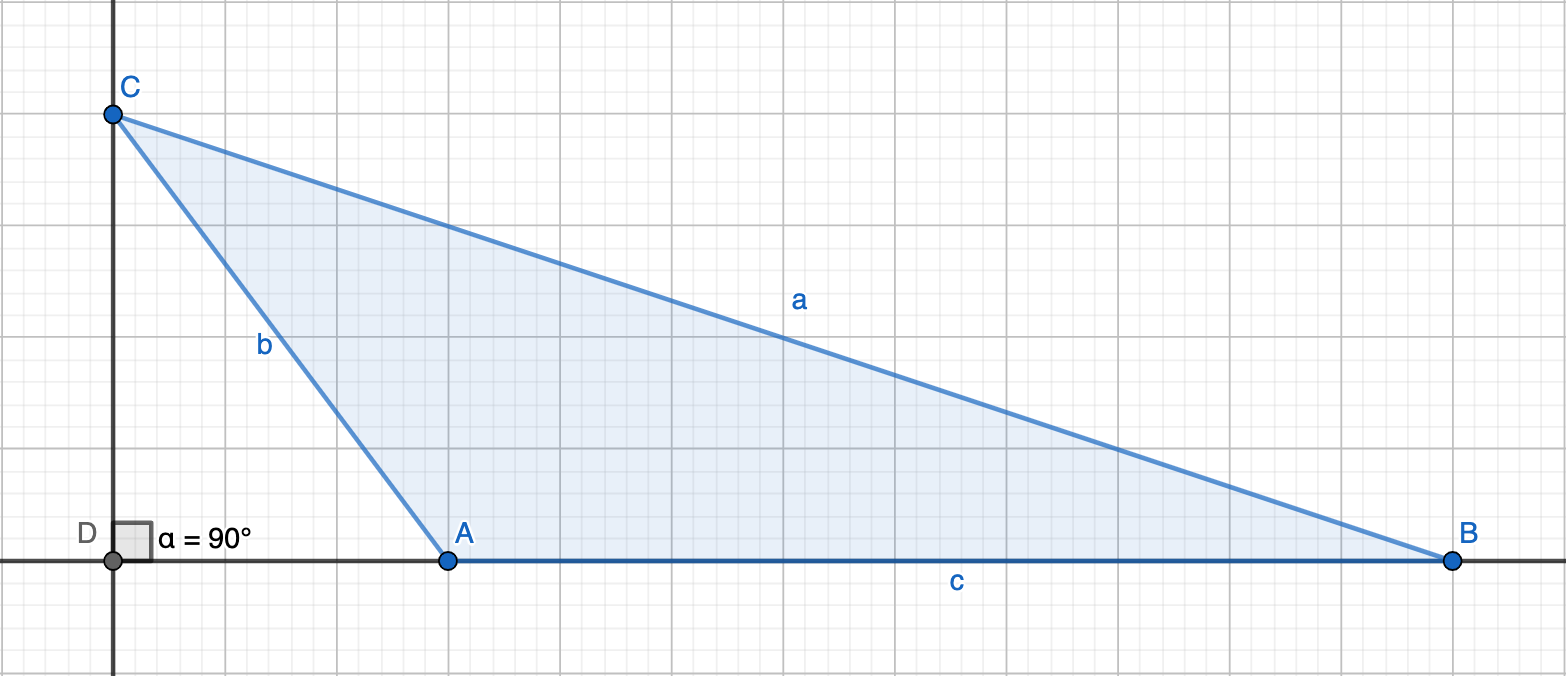
\includegraphics[width=0.8\linewidth]{Pythagorean_Obtuse.png}
			\end{figure}	
		\end{column}
	\end{columns}
\end{frame}
%------------------------------------------------

\begin{frame}
	\frametitle{Have a try!}
	\framesubtitle{}
In an obtuse triangle, if two sides are 9 and 40, what is range of the possible length of the unknown
one?\\ \pause

	\begin{columns}[t] 
		\begin{column}{0.25\textwidth} % Left column width

			\begin{equation*}
				\begin{aligned}
				& 40 - 9<x<40+9\\
				& 31 < x < 49\\
				& case \ 1: 40 \ is \ longest\\
				&31 < x \leq 40 \\
				& x^2 + 9^2 < 40^2 \\
				& 31 < x < 38.97 \\
				\end{aligned}
			\end{equation*}			
		\end{column}

				\begin{column}{0.25\textwidth} % Left column width

			\begin{equation*}
				\begin{aligned}
				& case \ 2: x \ is \ longest\\
				& 40 < x < 49 \\
				& 40^2 + 9^2 < x^2 \\
				& 41 < x  \\
				& 41 < x < 49 \\
				\end{aligned}
			\end{equation*}			
		Answer \textbf{$31 < x < 38.97 \ or\  41 < x < 49$}
		\end{column}

		\begin{column}{0.45\textwidth} % Right column width

		\pause
		\begin{figure}
			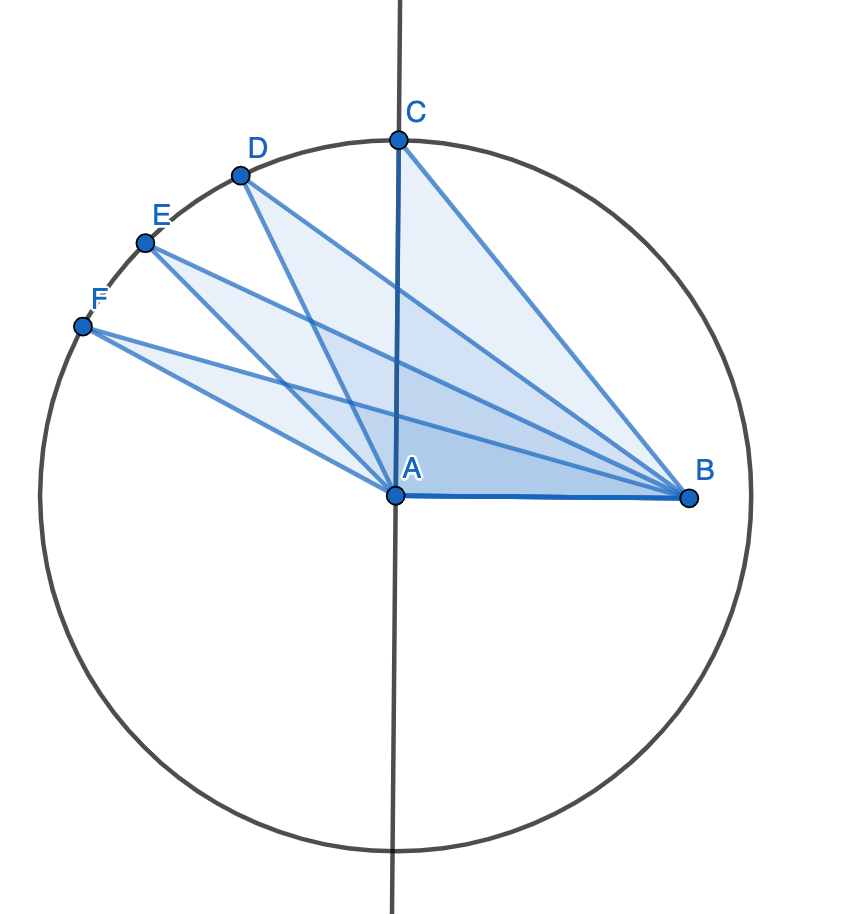
\includegraphics[width=\linewidth]{Pythagorean_Obtuse_Example_Question1.png}
		\end{figure}	

		\end{column}

	\end{columns}

\end{frame}

%------------------------------------------------

\begin{frame}
	\frametitle{The Pythagorean Inequality For The Acute Triangles} % Slide title, remove this command for no title
	\framesubtitle{锐角三角形长边任意两边平方和大于第三边}
	\begin{theorem}
	In an acute triangle, the sum of the square of two sides will be greater than the square of the the other side. 
	\end{theorem}
	\begin{columns}[t] 
		\begin{column}{0.4\textwidth} % Left column width
			\begin{equation*}
				\begin{aligned}
					&\because AE^2 + BE^2 = AB^2\\
					&\because BC^2 - CE^2 =BE^2 \\
					&\therefore (AE^2 - CE^2) + BC^2 = AB^2 \\
					&\therefore AC^2 + BC^2 \\
					&= (AE^2 +2AE*CE + CE^2) + BC^2 \\
					&> (AE^2 - CE^2) + BC^2 \\
					&=AB^2 \ Q.E.D.
				\end{aligned}
			\end{equation*}	
		\end{column}
		\begin{column}{0.6\textwidth} % Right column width
			\begin{figure}
				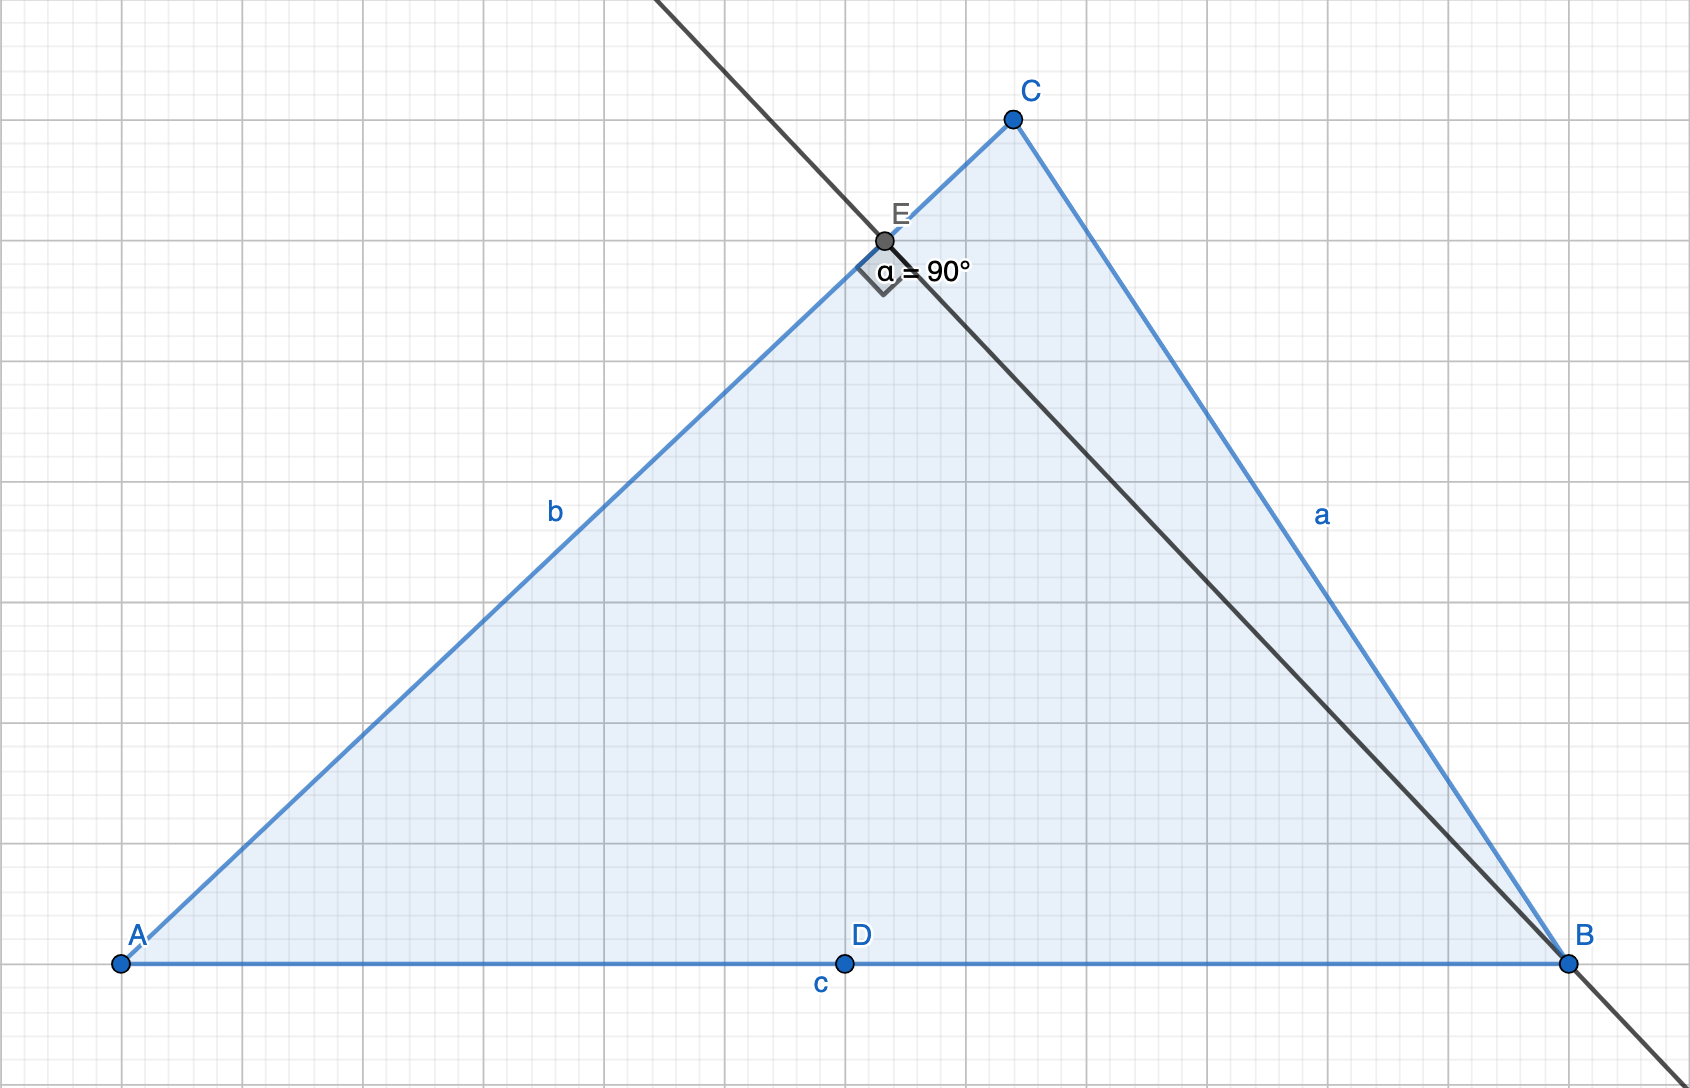
\includegraphics[width=0.8\linewidth]{Pythagorean_Acute.png}
			\end{figure}	
		\end{column}
	\end{columns}
\end{frame}

%------------------------------------------------

\begin{frame}
	\frametitle{Exterior Angle of Triangles} % Slide title, remove this command for no title
	\framesubtitle{外角等于相对应内对角之和}
		\begin{figure}
		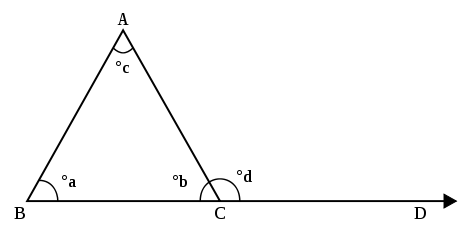
\includegraphics[width=0.5\linewidth]{Exterio_Angle.png}
	\end{figure}	
	\begin{theorem}
		\begin{equation*}
				d = a + c		
		\end{equation*}
	\end{theorem}
\end{frame}


%------------------------------------------------

\subsection{The Area of a Triangle}

%------------------------------------------------

\begin{frame}
	\frametitle{The Area of a Triangle} % Slide title, remove this command for no title
	\framesubtitle{底乘高除以二}
	\begin{figure}
		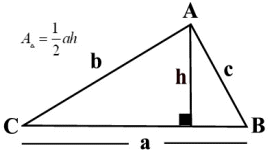
\includegraphics[width=0.5\linewidth]{Area_Triangle.png}
	\end{figure}	
\end{frame}

%------------------------------------------------

\subsection{Congruent Triangles}

%------------------------------------------------

\begin{frame}
	\frametitle{SSS, SAS, ASA Congruence} % Slide title, remove this command for no title
	\framesubtitle{边边边\ 边角边\ 角边角\ 全等}
			\begin{theorem}[Side-Side-Side Congruence]
				If the three sides of one triangle are congruent to the three
sides of another triangle, then the triangles are congruent.
			\end{theorem}

			\begin{theorem}[Side-Angle-Side Congruence]
				If two sides and the included angle of one triangle are
congruent to two sides and the included angle of another triangle,
then the triangles are congruent.
			\end{theorem}

			\begin{theorem}[Angle-Side-Angle Congruence]
				If two angles and the included side of one triangle are
congruent to two angles and the included side of another triangle,
then the triangles are congruent.
			\end{theorem}
What about AAS?\pause \alert{\textbf{Yes!}}
\end{frame}

%------------------------------------------------

\begin{frame}
	\frametitle{A Real QR Problem!}
	\framesubtitle{一个字!试!}
	\begin{figure}
		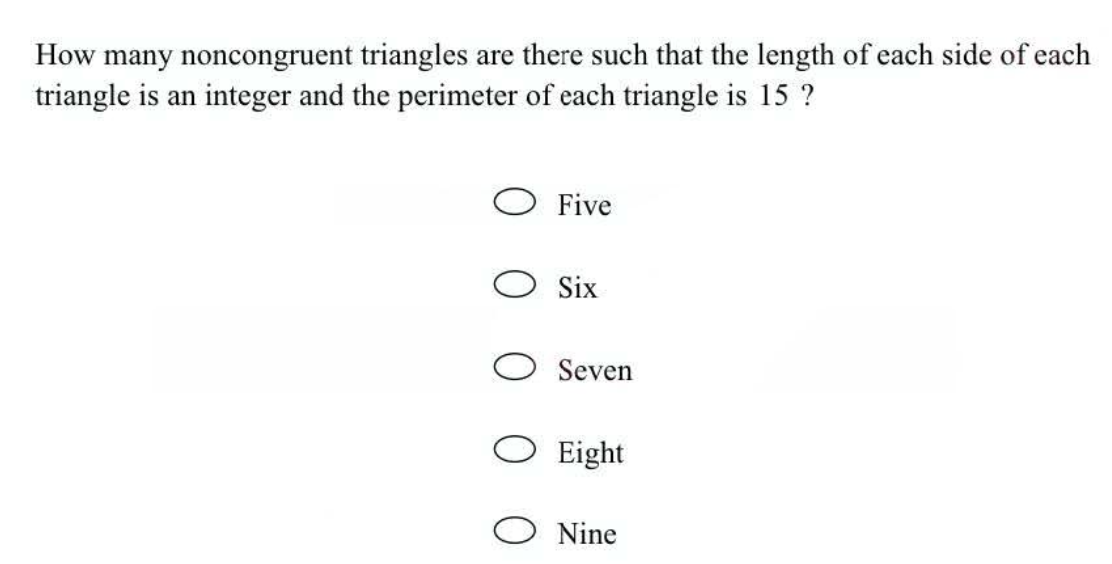
\includegraphics[width=\linewidth]{Triangle_Inequalities_Example_Question1.png}
		\caption{8-Sec2-12}
	\end{figure}
\end{frame}

%------------------------------------------------

\begin{frame}
	\frametitle{Answer}
	\framesubtitle{}
	\pause
		$a + b+ c = 15$\\
		$\because c< a+b = 15 - c$\\
		$\therefore c < 7.5$. By symmetry, $a<7.5$ and $b<7.5$\\
		The non-congruent triangles suggest that one triangle have different sides from other triangles.\\
		\begin{table}
			\begin{tabular}{l l l l}
				\toprule
				\textbf{c=7} &   \textbf{c=6}   & \textbf{c=5}    & \textbf{c=4}\\
				\textbf{a+b=7}&  \textbf{a+b=9} & \textbf{a+b=10} & \textbf{a+b=11}\\
				\midrule
				1\quad  7 & \Midline{1\quad   8} &\Midline{1\quad   9}  &\Midline{1\quad   10} \\
				2\quad  6 & \Midline{2\quad   7} &\Midline{2\quad   8}  &\Midline{2\quad   9} \\
				3\quad  5 & 3\quad   6           &\Midline{3\quad   7}  &\Midline{3\quad   8} \\
				4 \quad 4 & 4\quad   5           &\Midline{4\quad   6}  &\Midline{4\quad   7} \\
				$\ldots$  & $\ldots$             &5\quad   4  					&\Midline{5\quad   6} \\
				\bottomrule
			\end{tabular}
		\end{table}
		\pause
		Answer \textbf{C Seven}
\end{frame}

%------------------------------------------------


\subsection{Similar Triangles}

%------------------------------------------------

\begin{frame}
	\frametitle{Scale Factor Of Similarity} % Slide title, remove this command for no title
	\framesubtitle{相似比例}
		\begin{figure}
			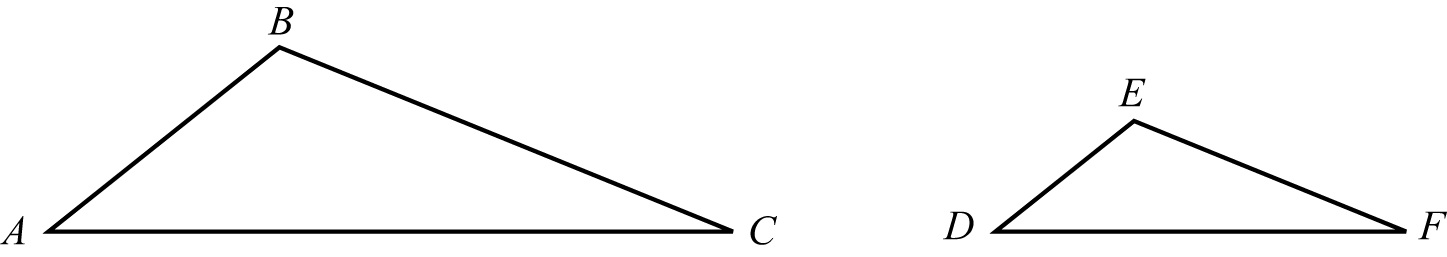
\includegraphics[width=0.8\linewidth]{Scale_Factor.jpg}
			\caption{Two similar triangles}
		\end{figure}
			\begin{definition}
				More precisely, two triangles are similar if their
vertices can be matched up so that the corresponding angles are congruent or,
equivalently, the lengths of the corresponding sides have the same ratio,
called \alert{the scale factor of similarity}.
			\end{definition}
How to prove similarity? \pause \alert{\textbf{AA!}}
\end{frame}

%------------------------------------------------

\begin{frame}
	\frametitle{Math Vocab!} % Slide title, remove this command for no title
	\framesubtitle{专业名词记忆时间!}
	
	{\Huge vertices}\\

		\bigskip\bigskip
	{\LARGE The plural noun of vertex \\ 
	顶点点的复数}

\end{frame}

%------------------------------------------------


\begin{frame}
	\frametitle{Have a try!}

In the figure shown below, fold the rectangle alone AF, and point D launch at E
which separate BC into two part. $BE = 6$, $EC = 2$. What is the value of $AE : EF$?\\ 
	\begin{columns}[t] 
		\begin{column}{0.3\textwidth} % Left column widt

		\begin{figure}
			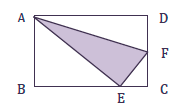
\includegraphics[width=\linewidth]{Similar_Triangle_Example_Question1.png}
			\pause
			Answer \textbf{$\frac{AE}{EF}\approx=2.65$}
		\end{figure}	
		\end{column}

		\begin{column}{0.7\textwidth} % Right column width
     \begin{equation*}
				\begin{aligned}
				&\because \angle FEC = \angle BAE \\ 
				& \ \angle BEA = \angle EFC\\
				& \therefore \triangle ABE \sim \triangle ECF\\
				& \therefore \frac{AE}{EF} = \frac{AB}{EC} = \frac{BE}{CF}\\
				& \because AE = AD = BC = BE + EC = 6 + 2 =8 \\
				&\therefore AB = \sqrt{AE^2 - BE^2}=\sqrt{8^2 - 6^2} = 2\sqrt{7} \\
				&\therefore \frac{AE}{EF}=\frac{AB}{EC}=\frac{2\sqrt{7}}{2}=\sqrt{7}\approx=2.65
				\end{aligned}
			\end{equation*}		
		\end{column}
	\end{columns}
\end{frame}

%------------------------------------------------


\begin{frame}
	\frametitle{A Real QR Problem!}
	\framesubtitle{}
	\begin{figure}
		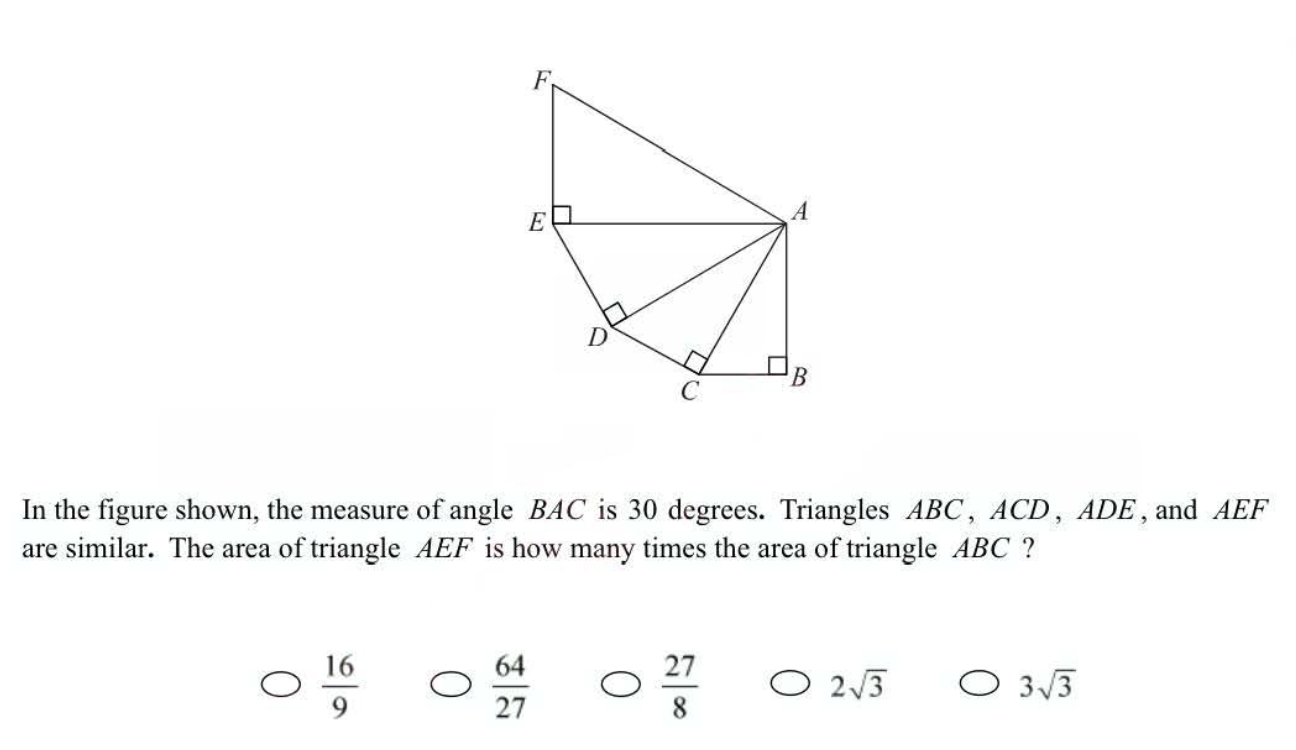
\includegraphics[width=\linewidth]{Similar_Triangle_Example_Question2.png}
		\caption{2-Sec2-18}
	\end{figure}
\end{frame}

%------------------------------------------------

\begin{frame}
	\frametitle{Answer}
	\framesubtitle{}
	\begin{columns}[t] 
		\begin{column}{0.3\textwidth} % Left column width
			\begin{figure}
				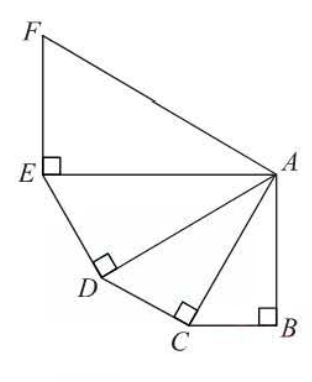
\includegraphics[width=\linewidth]{Similar_Triangle_Example_Question2_1.png}
			\end{figure}
			\pause
			Answer \textbf{B $\frac{64}{27}$}		
		\end{column}
		\begin{column}{0.7\textwidth} % Right column width
			\pause
	     \begin{equation*}
					\begin{aligned}
					BC &= x\\
					DC &= \frac{1}{\sqrt{3}} AC = \frac{2}{\sqrt{3}} x\\
					DE &= \frac{1}{\sqrt{3}} AD = \frac{1}{\sqrt{3}}\frac{4}{\sqrt{3}} x
					   = \frac{4}{3} x \\
					EF &= \frac{1}{\sqrt{3}} AE = \frac{1}{\sqrt{3}} \frac{8}{3} x =
					   \frac{8}{3\sqrt{3}} x\\
					\frac{S_{\triangle AFE}}{S_{\triangle ABC}} &= \frac{\frac{\sqrt{3}}{2}EF^2}{\frac{\sqrt{3}}{2}BC^2}
					   = (\frac{EF}{BC})^2 = (\frac{\frac{8}{3\sqrt{3}} x}{x})^2 
					   = \frac{64}{27}
					\end{aligned}
				\end{equation*}					
		\end{column}
	\end{columns}
\end{frame}

%------------------------------------------------


\section{Quadrilaterals}

%------------------------------------------------

\begin{frame}
	\frametitle{Math Vocab!} % Slide title, remove this command for no title
	\framesubtitle{专业名词记忆时间!}
	
	{\Huge quadrilateral}\\
	{\LARGE /ˌkwädrəˈladərəl,ˌkwädrəˈlatrəl/\\
		\bigskip\bigskip
	a four-sided figure. \\ 
	四边形}

\end{frame}

%------------------------------------------------

\subsection{Rectangle}

%------------------------------------------------

\begin{frame}
	\frametitle{Rectangle} % Slide title, remove this command for no title
	\framesubtitle{矩形}
	\begin{definition}
		A quadrilateral with four right angles is called a rectangle.
Opposite sides of a rectangle are parallel and congruent, and the two
diagonals are also congruent. \\
A rectangle with four congruent sides is called a square.
	\end{definition}

	\begin{columns}[t] 
		\begin{column}{0.5\textwidth} % Left column width
			\begin{figure}
				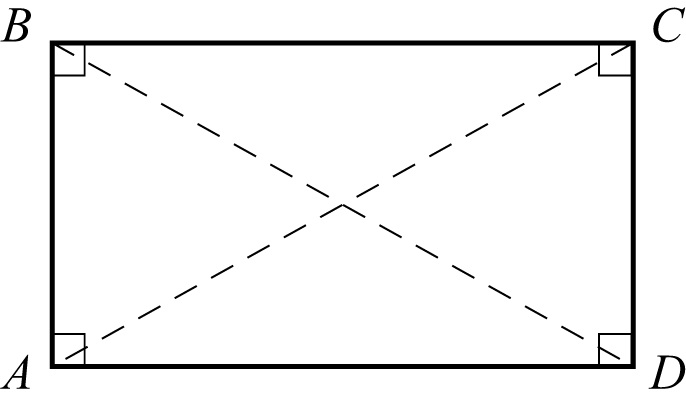
\includegraphics[width=\linewidth]{Retangle.jpg}
			\end{figure}
		\end{column}
		\begin{column}{0.5\textwidth} % Right column width
			\begin{equation*}
				Area:\ A = base \cdot height
			\end{equation*}
		\end{column}
	\end{columns}
\end{frame}

%------------------------------------------------

\subsection{Parallelogram}

%------------------------------------------------

\begin{frame}
	\frametitle{Math Vocab!} % Slide title, remove this command for no title
	\framesubtitle{专业名词记忆时间!}
	
	{\Huge parallelogram}\\
	{\LARGE /ˌperəˈleləˌɡram/\\
		\bigskip\bigskip
	a four-sided plane rectilinear figure with opposite sides parallel. \\ 
	平行四边形}

\end{frame}

%------------------------------------------------
	\begin{frame}
	\frametitle{Parallelogram} % Slide title, remove this command for no title
	\framesubtitle{平行四边形}
	\begin{definition}
		A quadrilateral in which both pairs of opposite sides are parallel
		is called a parallelogram. In a parallelogram, opposite sides are
		congruent and opposite angles are congruent. \\
		Note that all rectangles are parallelograms.
	\end{definition}

	\begin{columns}[t] 
		\begin{column}{0.5\textwidth} % Left column width
			\begin{figure}
				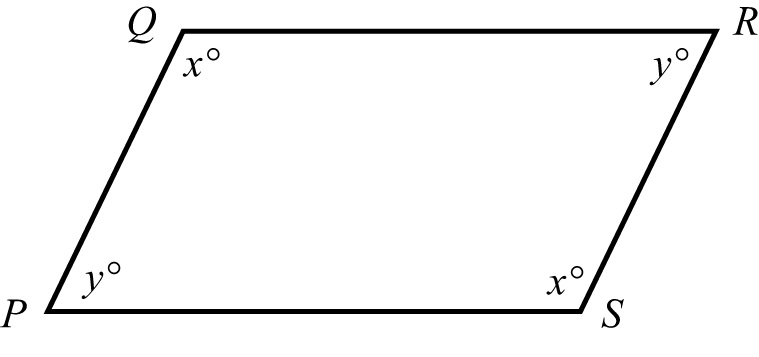
\includegraphics[width=\linewidth]{Parallelogram.jpg}
			\end{figure}
		\end{column}

		\begin{column}{0.5\textwidth} % Right column width
			\begin{equation*}
				Area:\ A = base \cdot height
			\end{equation*}
		\end{column}
	\end{columns}
\end{frame}

%------------------------------------------------

\subsection{Trapezoid}

%------------------------------------------------

\begin{frame}
	\frametitle{Math Vocab!} % Slide title, remove this command for no title
	\framesubtitle{专业名词记忆时间!}
	
	{\Huge trapezoid}\\
	{\LARGE /ˈtrapɪzɔɪd,trəˈpiːzɔɪd/\\
		\bigskip\bigskip
	a four-sided plane rectilinear figure with opposite sides parallel. \\ 
	梯形}

\end{frame}

%------------------------------------------------
	\begin{frame}
	\frametitle{Trapezoid} % Slide title, remove this command for no title
	\framesubtitle{梯形}
	\begin{definition}
A quadrilateral in which at least one pair of opposite sides is
parallel is called a trapezoid. \\
Two opposite, parallel sides of the
trapezoid are called bases of the trapezoid.
	\end{definition}

	\begin{columns}[t] 
		\begin{column}{0.5\textwidth} % Left column width
			\begin{figure}
				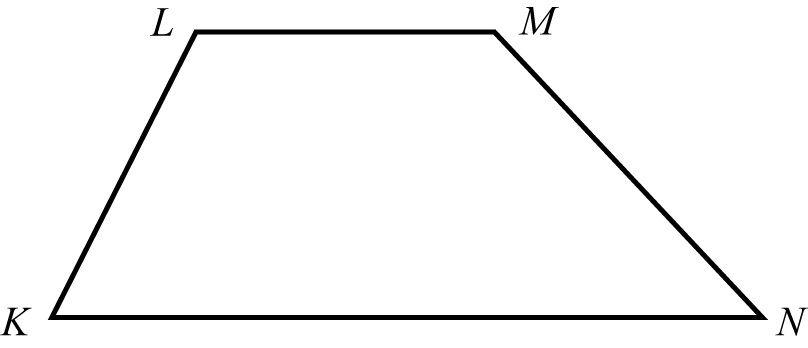
\includegraphics[width=\linewidth]{trapezoid.jpg}
			\end{figure}
		\end{column}

		\begin{column}{0.5\textwidth} % Right column width
			\begin{equation*}
				Area:\ A = \frac{base_1 + base_2}{2}\cdot height
			\end{equation*}
		\end{column}
	\end{columns}
\end{frame}

%------------------------------------------------


\begin{frame}
	\frametitle{A Real QR Problem!}
	\framesubtitle{自己画图!}
	\begin{figure}
		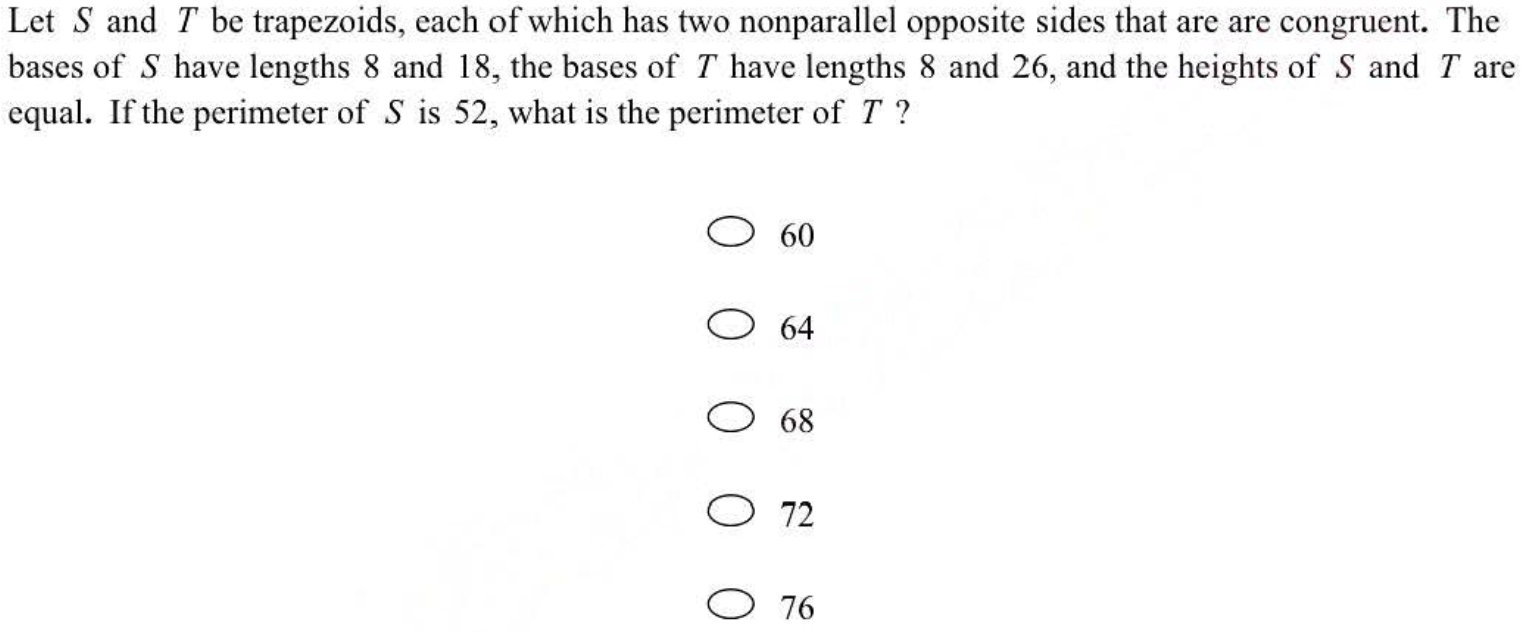
\includegraphics[width=\linewidth]{Trapezoid_Question1.png}
		\caption{5-Sec2-13}
	\end{figure}
\end{frame}

%------------------------------------------------


\begin{frame}
	\frametitle{Answer}
	\begin{columns}[t] 

		\begin{column}{0.5\textwidth} % Left column width
		  \pause
			\begin{figure}
				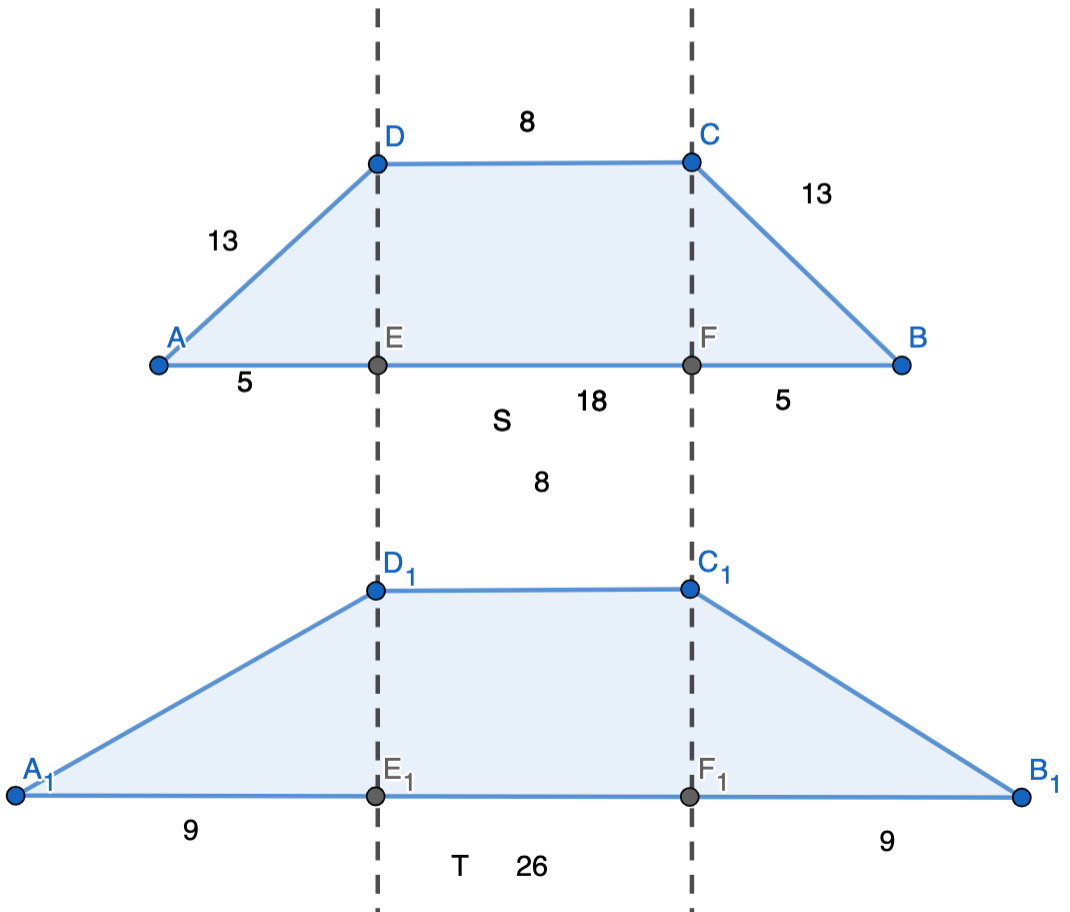
\includegraphics[width=\linewidth]{Trapezoid_Question1_1.png}
			\end{figure}
		\end{column}

		\begin{column}{0.5\textwidth} % Right column width
			\begin{equation*}
				\begin{aligned}
					&AD= CB = \frac{perimeter_S - DC - AB}{2}\\
					&=\frac{52 - 8 - 18}{2}=13\\
					&\because congruent\ nonparallel\ sides\\
					&\therefore  AD  = BC\\
					&\therefore AE  = BF = \frac{AB - CD}{2}\\
					&=\frac{18 - 8}{2}=5\\
					&DE=CF = \sqrt{AD^2 - AE^2} \\
					&=\sqrt{13^2 - 5^2} =12\\
				\end{aligned}
			\end{equation*}	
		\end{column}

	\end{columns}
\end{frame}

%------------------------------------------------


\begin{frame}
	\frametitle{Answer}
	\begin{columns}[t] 

		\begin{column}{0.5\textwidth} % Left column width
		  \pause
			\begin{figure}
				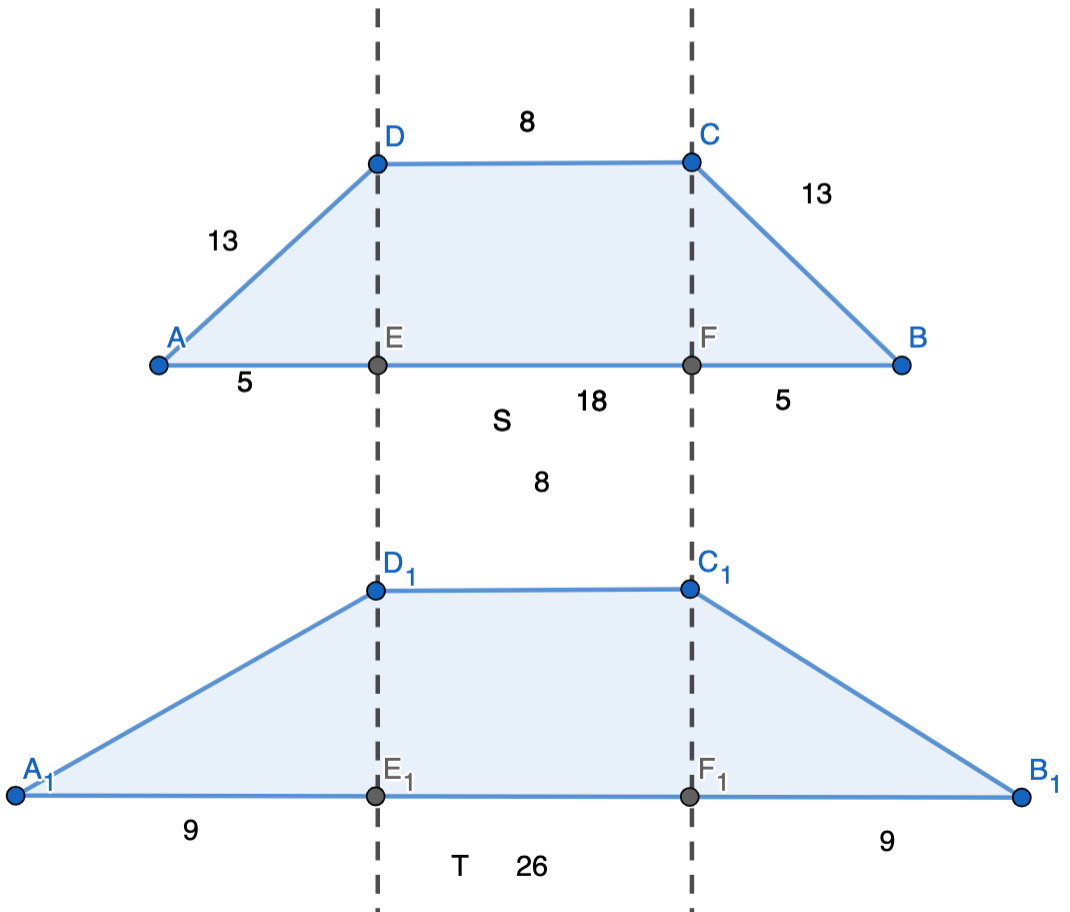
\includegraphics[width=\linewidth]{Trapezoid_Question1_1.png}
			\end{figure}
		 	 Answer \textbf{B} 64
		\end{column}

		\begin{column}{0.5\textwidth} % Right column width
			\begin{equation*}
				\begin{aligned}
					&\because same height\\
					& \therefore DE = CF = D_1E_1 = C_1F_1 =12\\
					&\because congruent\ nonparallel\ sides\\
					&\therefore  A_1D_1  = B_1C_1\\
					&\therefore A_1E_1  = B_1F_1 = \frac{A_1B_1 - C_1D_1}{2}\\
					&=\frac{26 - 8}{2}=9\\
					& \therefore A_1D_1 =B_1C_1= \sqrt{D_1E_1^2 + A_1E_1^2}\\
					&= \sqrt{12^2 + 9^2}= 15\\
				  &\therefore perimeter_T = 2A_1D_1 + D_1C_1 + A_1 + B_1\\
				  &= 2\cdot 15 + 8 + 26 = 64
				\end{aligned}
			\end{equation*}	
		\end{column}

	\end{columns}
\end{frame}

%------------------------------------------------
\section{Circles}

%------------------------------------------------

\subsection{Radius, Diameter, And Chord}

%------------------------------------------------

\begin{frame}
	\frametitle{Radius, Diameter, And Chord} % Slide title, remove this command for no title
	\framesubtitle{半径\ 直径\ 弦}
			\begin{columns}[t] 
				\begin{column}{0.4\textwidth} % Left column width
					\begin{figure}
						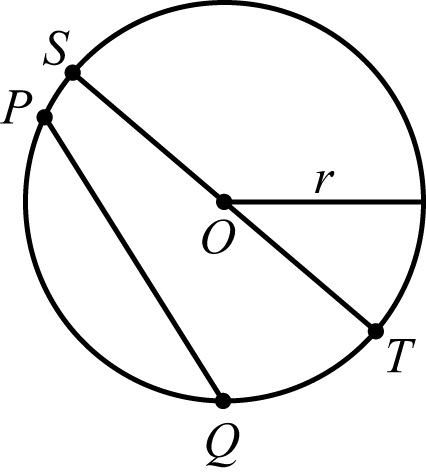
\includegraphics[width=\linewidth]{Radius_Diameter_Chord.jpg}
						\caption{r is the radius; $PQ$ is the chord; ST is the diameter as well as the chord.}
					\end{figure}

				\end{column}
				\begin{column}{0.6\textwidth} % Right column width

				\begin{definition}
				The point O is
		called the center of the circle and the distance r is called the radius of the
		circle.\\
		The diameter of the circle is twice the radius.\\
		Two circles with equal radii are called congruent circles.
				\end{definition}
				\end{column}
			\end{columns}

\end{frame}

%------------------------------------------------

\begin{frame}
	\frametitle{Math Vocab!} % Slide title, remove this command for no title
	\framesubtitle{专业名词记忆时间!}
	
	{\Huge radii}\\

		\bigskip\bigskip
		{\LARGE The plural noun of radius \\ 
		半径的复数}

\end{frame}

%------------------------------------------------



\subsection{Circumference,Area, Central Angle and Arc}
%圆心角是圆周角的两倍
%
%------------------------------------------------

\begin{frame}
\frametitle{Circumference and Area}
\framesubtitle{周长和面积计算公式}
\begin{equation*}
\begin{aligned}
	c &= 2\pi r \\
	A &= \pi r^2
\end{aligned}
\end{equation*}

\bigskip\bigskip\bigskip\bigskip
\alert{$\pi$取3.14或者$\frac{22}{7}$}
\end{frame}

%------------------------------------------------

\begin{frame}
\frametitle{Central Angle and Arc}
\framesubtitle{圆心角和弧}

\begin{columns}[t] 
		\begin{column}{0.4\textwidth} % Left column width
			\begin{figure}
				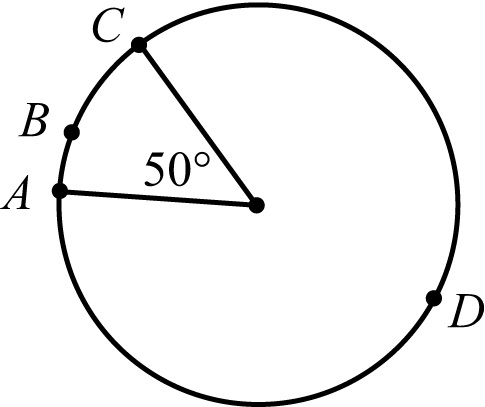
\includegraphics[width=\linewidth]{Central_Angle_Arc.jpg}
				\caption{The measure of an arc is the measure of its central angle, which is the
angle formed by two radii that connect the center of the circle to the two
endpoints of the arc.}
			\end{figure}

		\end{column}
		\begin{column}{0.6\textwidth} % Right column width
			\begin{equation*}
			\begin{aligned}
				length\ of \ the \ arc &= 2\pi r \frac{360}{central\ angle}\\
				sector\ area  &= \pi r^2 \frac{360}{central\ angle}
			\end{aligned}
			\end{equation*}
		\end{column}
	\end{columns}
\end{frame}

%------------------------------------------------


\begin{frame}
\frametitle{Central Angle Property}
\framesubtitle{圆心角是圆周角的两倍}

\begin{columns}[t] 
		\begin{column}{0.4\textwidth} % Left column width
			\begin{figure}
				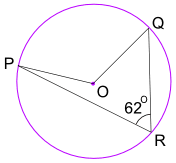
\includegraphics[width=\linewidth]{Central_Angle_Property.png}
				\caption{Angle POQ is the central angle of arc PQ; angle PRQ is the inscribed angle of the arc PQ;$\angle\ POQ = 2\cdot \angle PRQ$ }
			\end{figure}

		\end{column}
		\begin{column}{0.6\textwidth} % Right column width

		\begin{theorem}
			An inscribed angle is half the measure of a central angle subtended by the same arc.
		\end{theorem}
		\end{column}
	\end{columns}
\end{frame}

%------------------------------------------------

\begin{frame}
\frametitle{The Proof of Central Angle Property}
\framesubtitle{圆周角圆心角关系证明}

\begin{columns}[t] 
		\begin{column}{0.4\textwidth} % Left column width
			\begin{equation*}
			\begin{aligned}
			&By\ the\ property\ of\ exterior\ \\&angles\ of\ triangles,\\
			&\angle CAF = \angle ACE + \angle CEA\\
			&\angle FAD = \angle AED + \angle ADE\\
			&\because AC = AE  = r\\
			&\therefore \angle ACE = \angle CEA\\
			&\because AD = AE  = r\\
			&\therefore \angle AED = \angle ADE\\
			&\therefore \angle CAD = \angle CAF + \angle FAD\\
			&= 2(\angle CEA + \angle AED)\\
			&= 2 \angle CED\ Q.E.D.
			\end{aligned}
			\end{equation*}
		\end{column}
		\begin{column}{0.6\textwidth} % Right column width
			\begin{figure}
				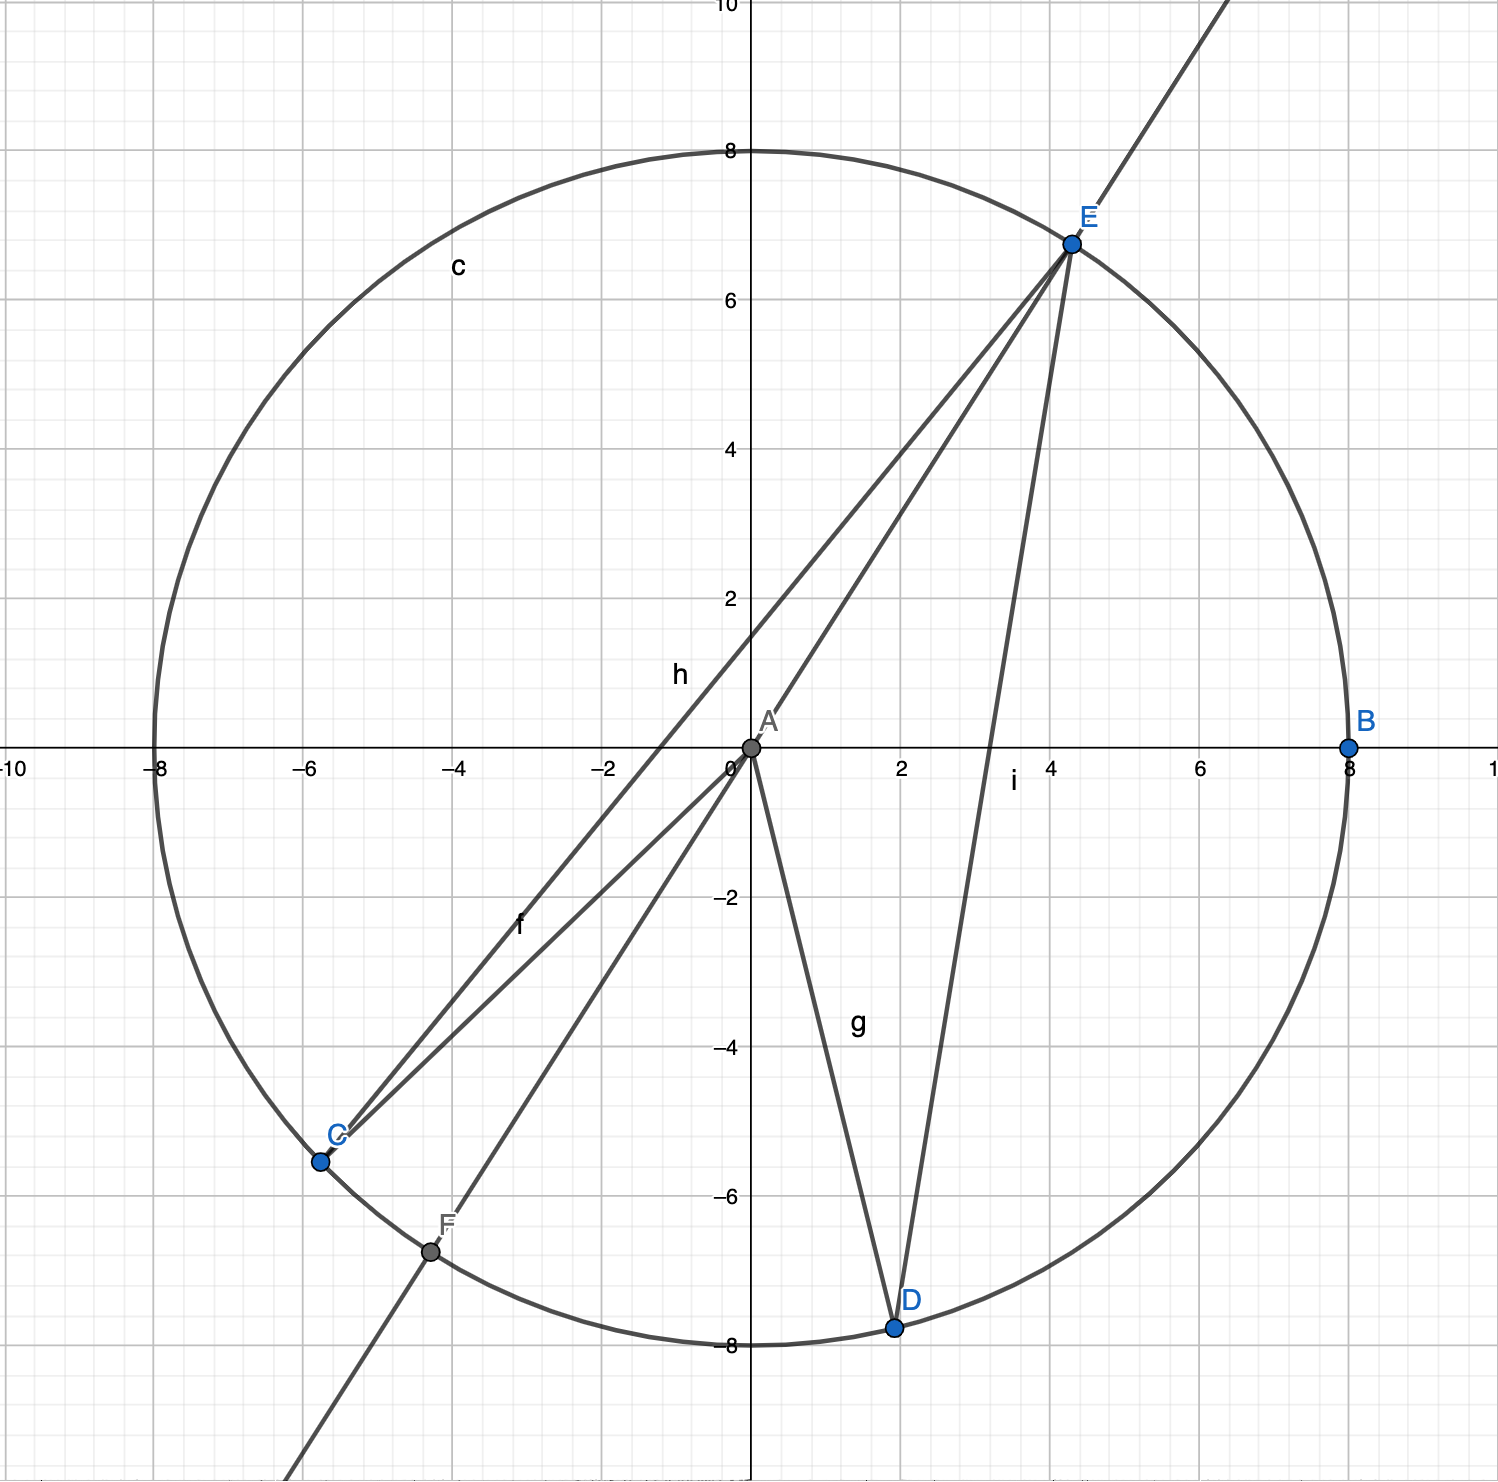
\includegraphics[width=\linewidth]{Proof_Central_Angle_Property.png}
			\end{figure}
		\end{column}
	\end{columns}
\end{frame}

%------------------------------------------------


%------------------------------------------------

\begin{frame}
\frametitle{The Proof of Inscribed Angle Property}
\framesubtitle{相同弧圆周角相同}

\begin{columns}[t] 
		\begin{column}{0.4\textwidth} % Left column width
			\begin{equation*}
			\begin{aligned}
			&By\ the\ property\ of\ central\ \\
			&angles\ of\ triangles,\\
			&\angle CFD = \frac{1}{2}\angle CAD = \angle CED 
			\end{aligned}
			\end{equation*}
		\end{column}
		\begin{column}{0.6\textwidth} % Right column width
			\begin{figure}
				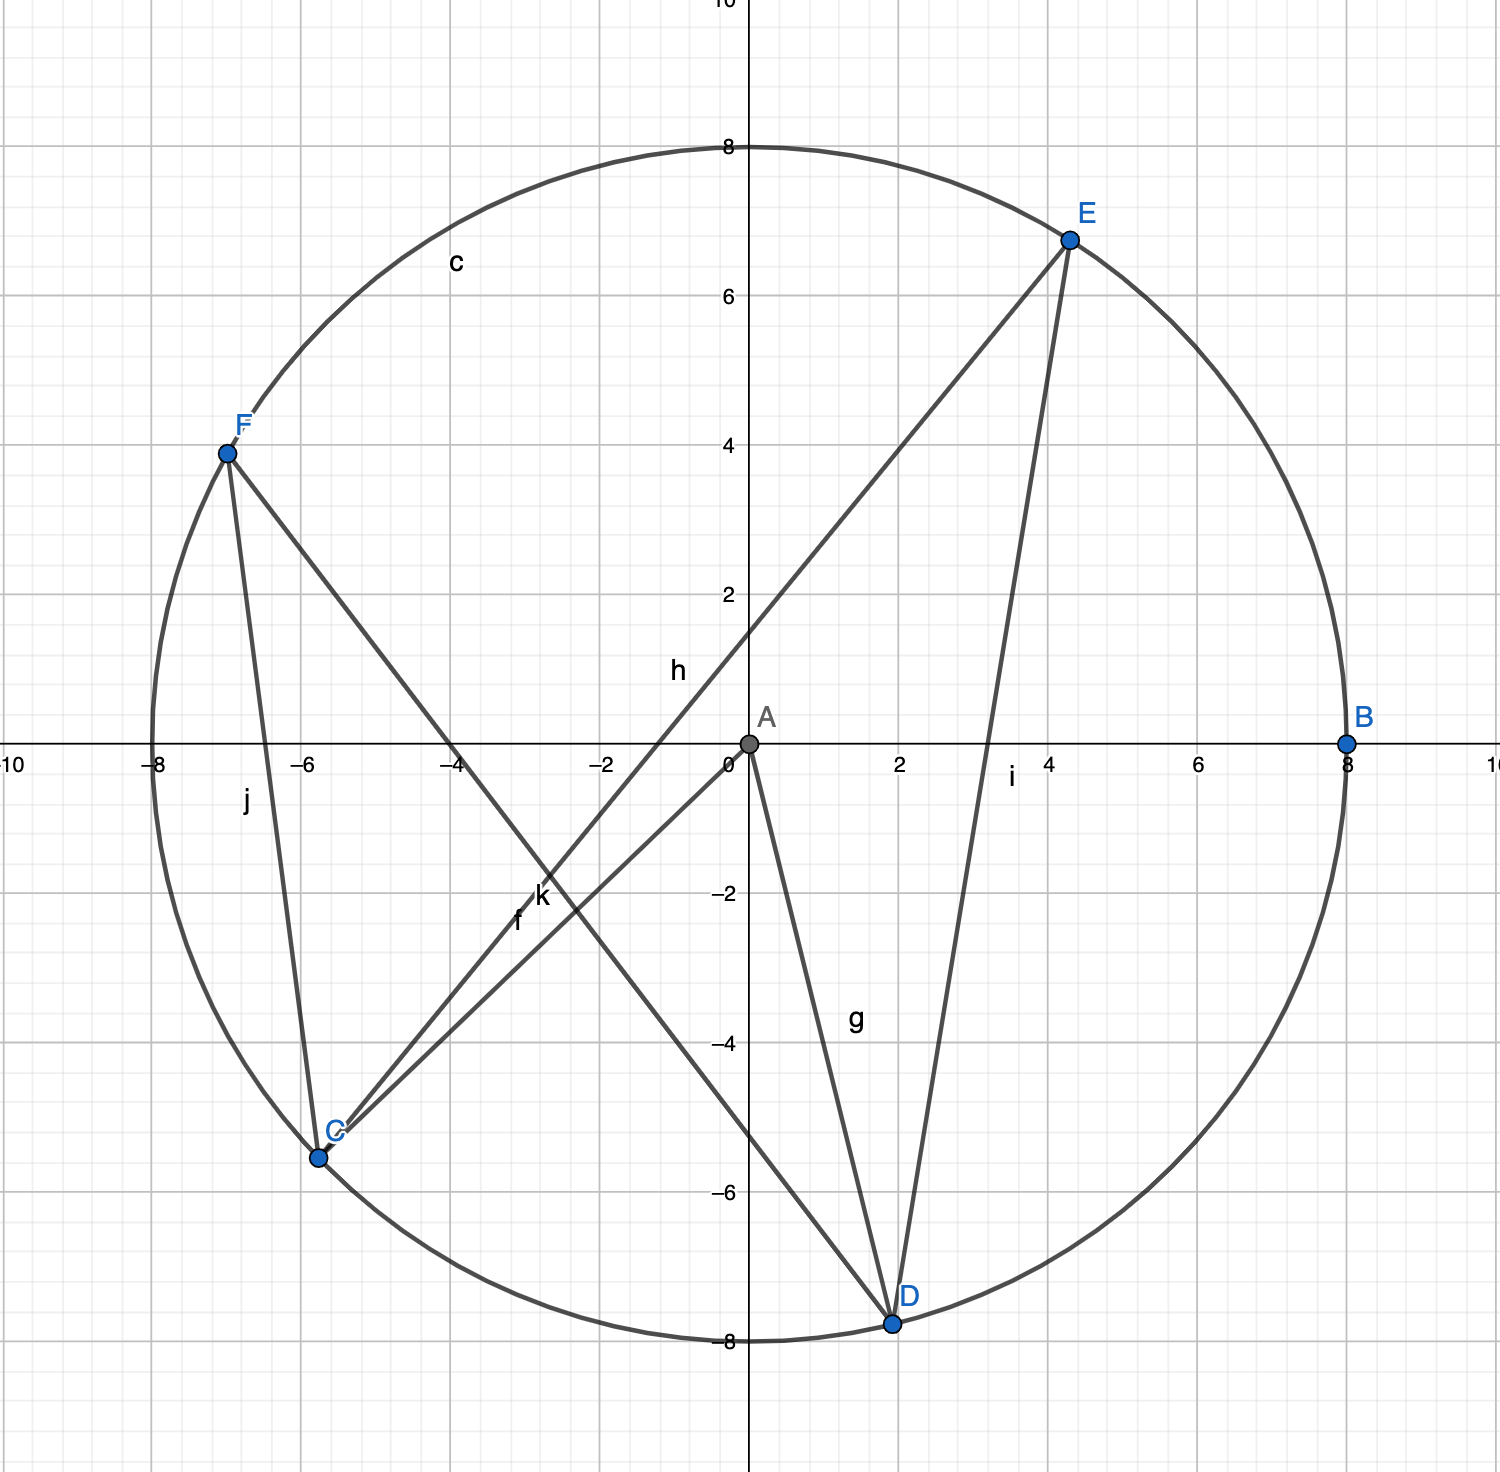
\includegraphics[width=\linewidth]{Inscribed_Angle.png}
			\end{figure}
		\end{column}
	\end{columns}
\end{frame}

%------------------------------------------------

\subsection{Tangent}

%------------------------------------------------

\begin{frame}
	\frametitle{Tangent} % Slide title, remove this command for no title
	\framesubtitle{切线}
			\begin{columns}[t] 
				\begin{column}{0.4\textwidth} % Left column width
					\begin{figure}
						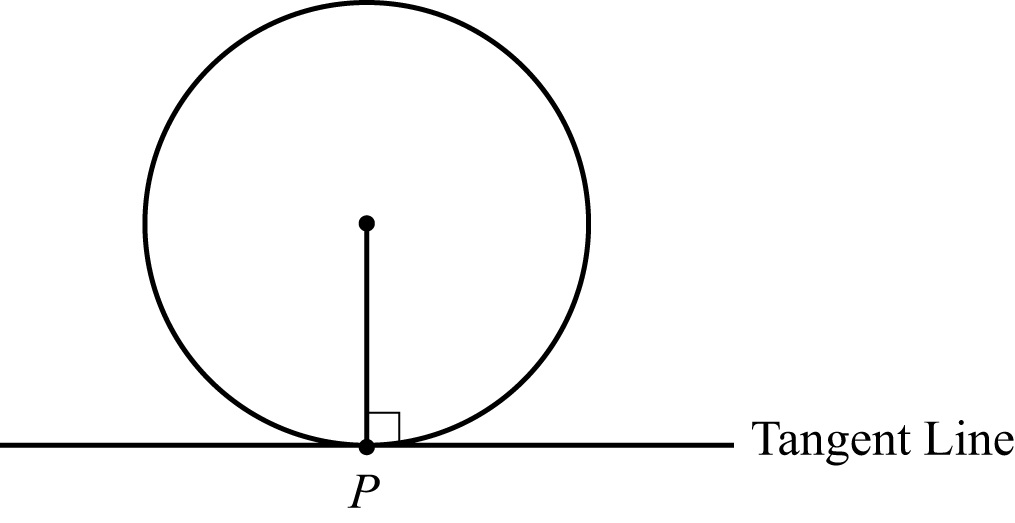
\includegraphics[width=\linewidth]{Tangent.jpg}
						\caption{$\angle p = \ang{90}$}
					\end{figure}

				\end{column}
				\begin{column}{0.6\textwidth} % Right column width

				\begin{definition}
	A tangent to a circle is a line that lies in the same plane as the circle and
intersects the circle at exactly one point, called the point of tangency
				\end{definition}
				\begin{theorem}[切线和交点半径垂直]
					that is, if a radius
and a line intersect at a point on the circle and the line is perpendicular to the
radius, then the line is a tangent to the circle at the point of intersection.
				\end{theorem}
				\end{column}
			\end{columns}
\end{frame}

%------------------------------------------------

\begin{frame}
	\frametitle{Have a try!}
	\framesubtitle{自己用手画图!}
In the rectangular coordinate system below, both of two tangent circles are tangent
to the x-axis. If the radii of the two circles are 4 and 6, respectively, what is the slope
of the line on which two centers lie?\\


		\begin{figure}
			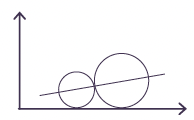
\includegraphics[width=0.5\linewidth]{Tangent_Example_Question1.png}
		\end{figure}	


\end{frame}

%------------------------------------------------

\begin{frame}
	\frametitle{Have a try!}
	\framesubtitle{自己用手画图!}
\begin{columns}[t] 
	\begin{column}{0.55\textwidth} % Left column width
		\begin{figure}
			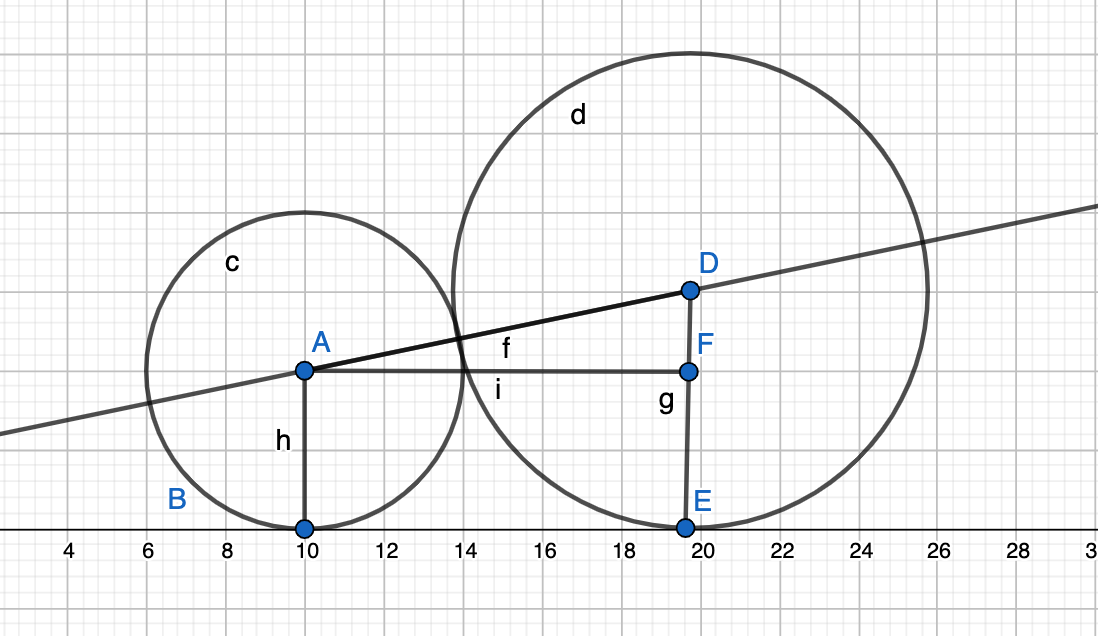
\includegraphics[width=\linewidth]{Tangent_Example_Question1_1.png}
		\end{figure}	
	\end{column}

	\begin{column}{0.545\textwidth} % Right column width
	\pause
	\begin{equation*}
		\begin{aligned}
		&slope=\frac{DF}{AF}\\
		&=\frac{DE - AB}{\sqrt{AD^2 - DF^2}}\\
		&= \frac{6 - 4}{\sqrt{10^2 - 2^2}}\\
		&=\frac{2}{\sqrt{96}}\\
		&=0.20
		\end{aligned}
	\end{equation*}
	\bigskip
	Answer \textbf{0.20}
	\end{column}

\end{columns}
\end{frame}

%------------------------------------------------



\begin{frame}
	\frametitle{A Real QR Problem!}
	\framesubtitle{}
	\begin{figure}
		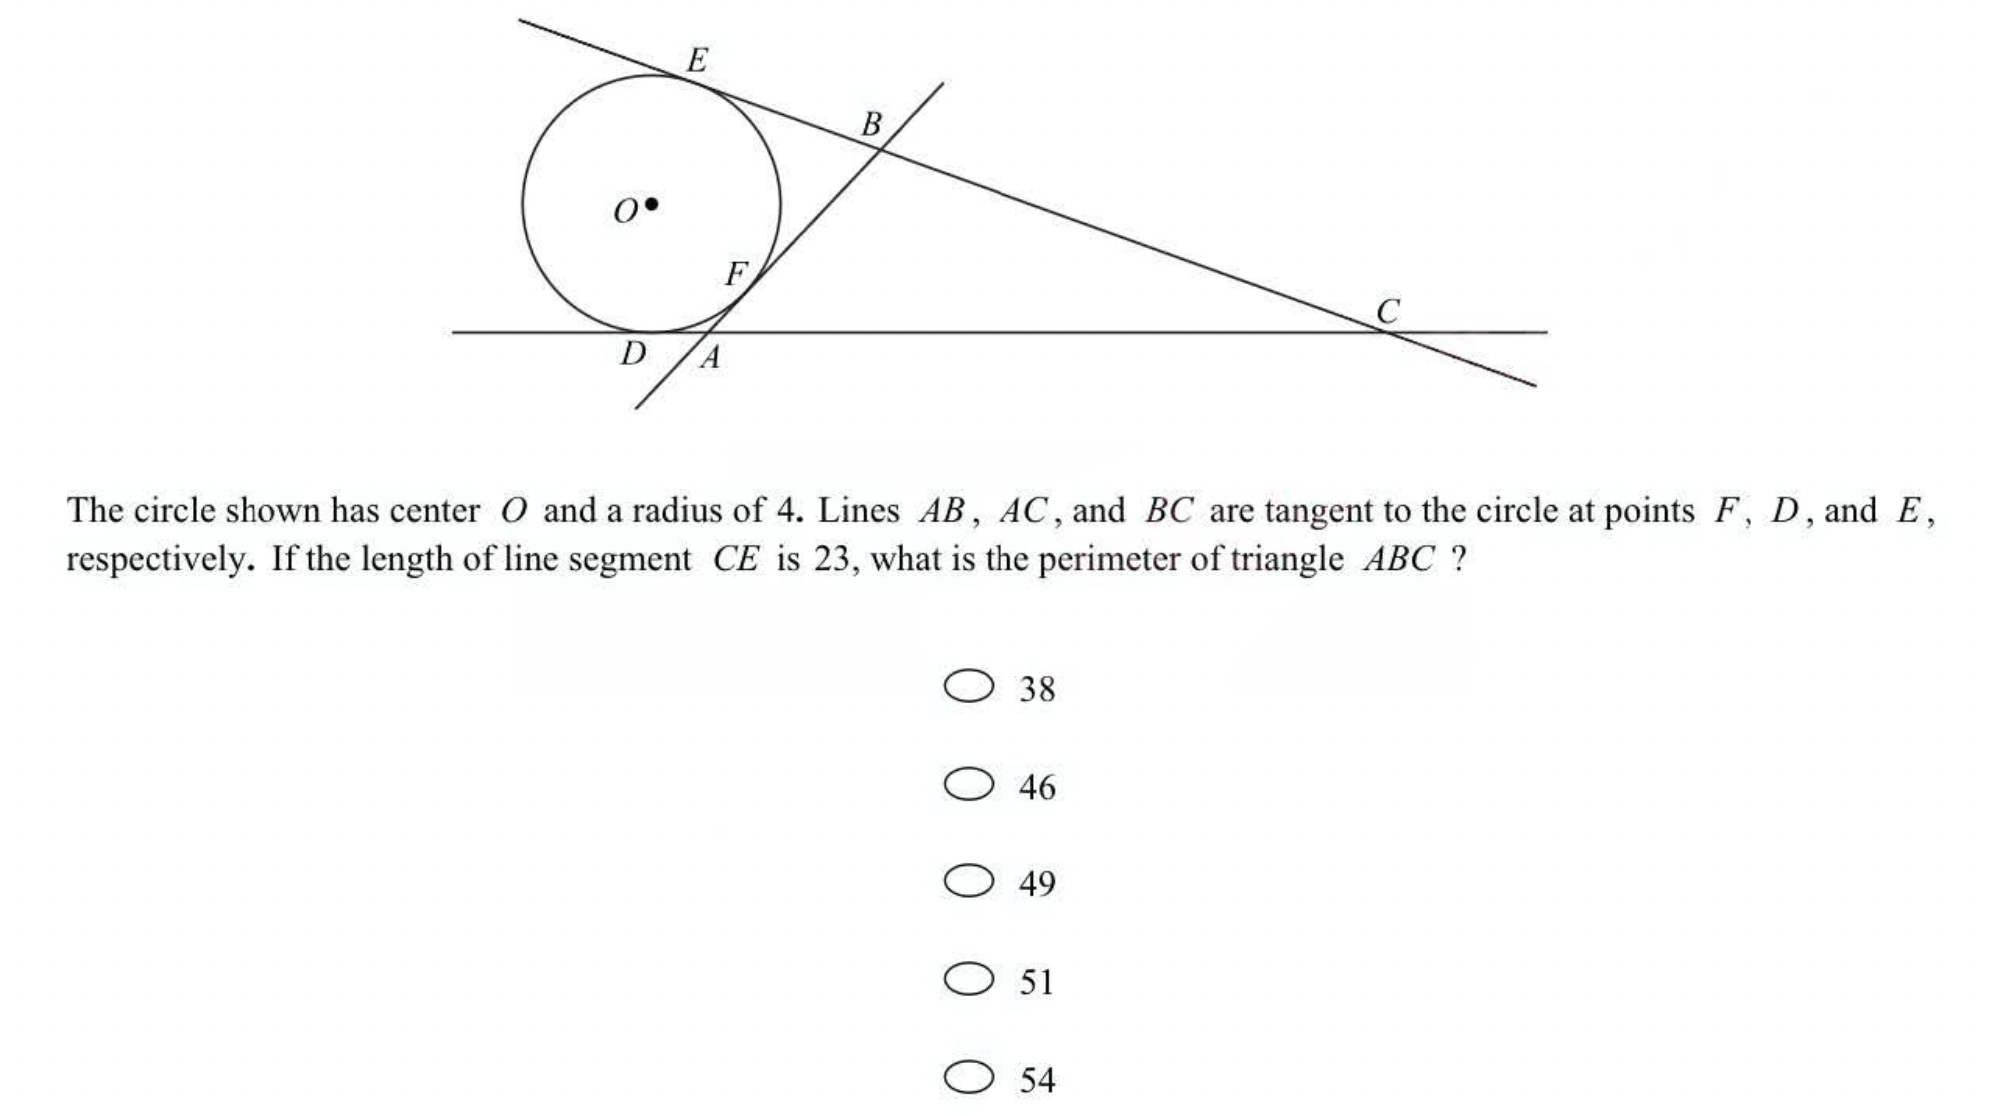
\includegraphics[width=0.8\linewidth]{Tangent_Example_Question2.png}
		\caption{7-Sec2-13}
	\end{figure}
\end{frame}

%------------------------------------------------

\begin{frame}
	\frametitle{Answer}
	\framesubtitle{}
			\begin{figure}
				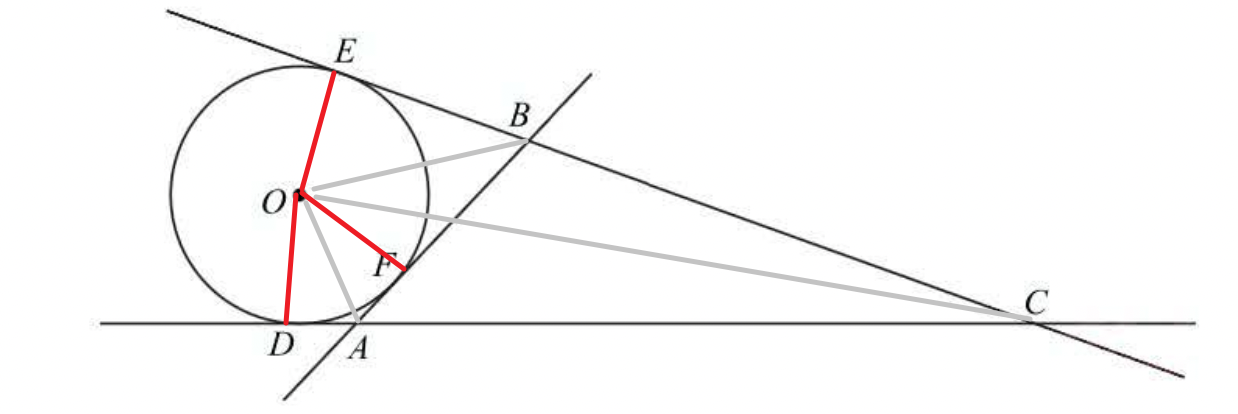
\includegraphics[width=0.7\linewidth]{Tangent_Example_Question2_1.png}
			\end{figure}
			\pause
	     \begin{equation*}
					\begin{aligned}
					&By\ symmetry, BE = BF\ AD = AF\ CE = CD\\
					&Perimeter_{\triangle ABC} = AB + BC + AC\\
					&=(BC + BF) + (AF + AC)\\
					&=(BC + BE) + (AD + AC)\\
					&=CE + AC = 2AE = 2\cdot 23 = 46
					\end{aligned}
				\end{equation*}					
			\pause
			Answer \textbf{B $46$}
\end{frame}

%------------------------------------------------

\begin{frame}
\frametitle{Chord Tangent Angle Property}
\framesubtitle{弦切角圆周角相等}

\begin{columns}[t] 
		\begin{column}{0.4\textwidth} % Left column width
			\begin{figure}
				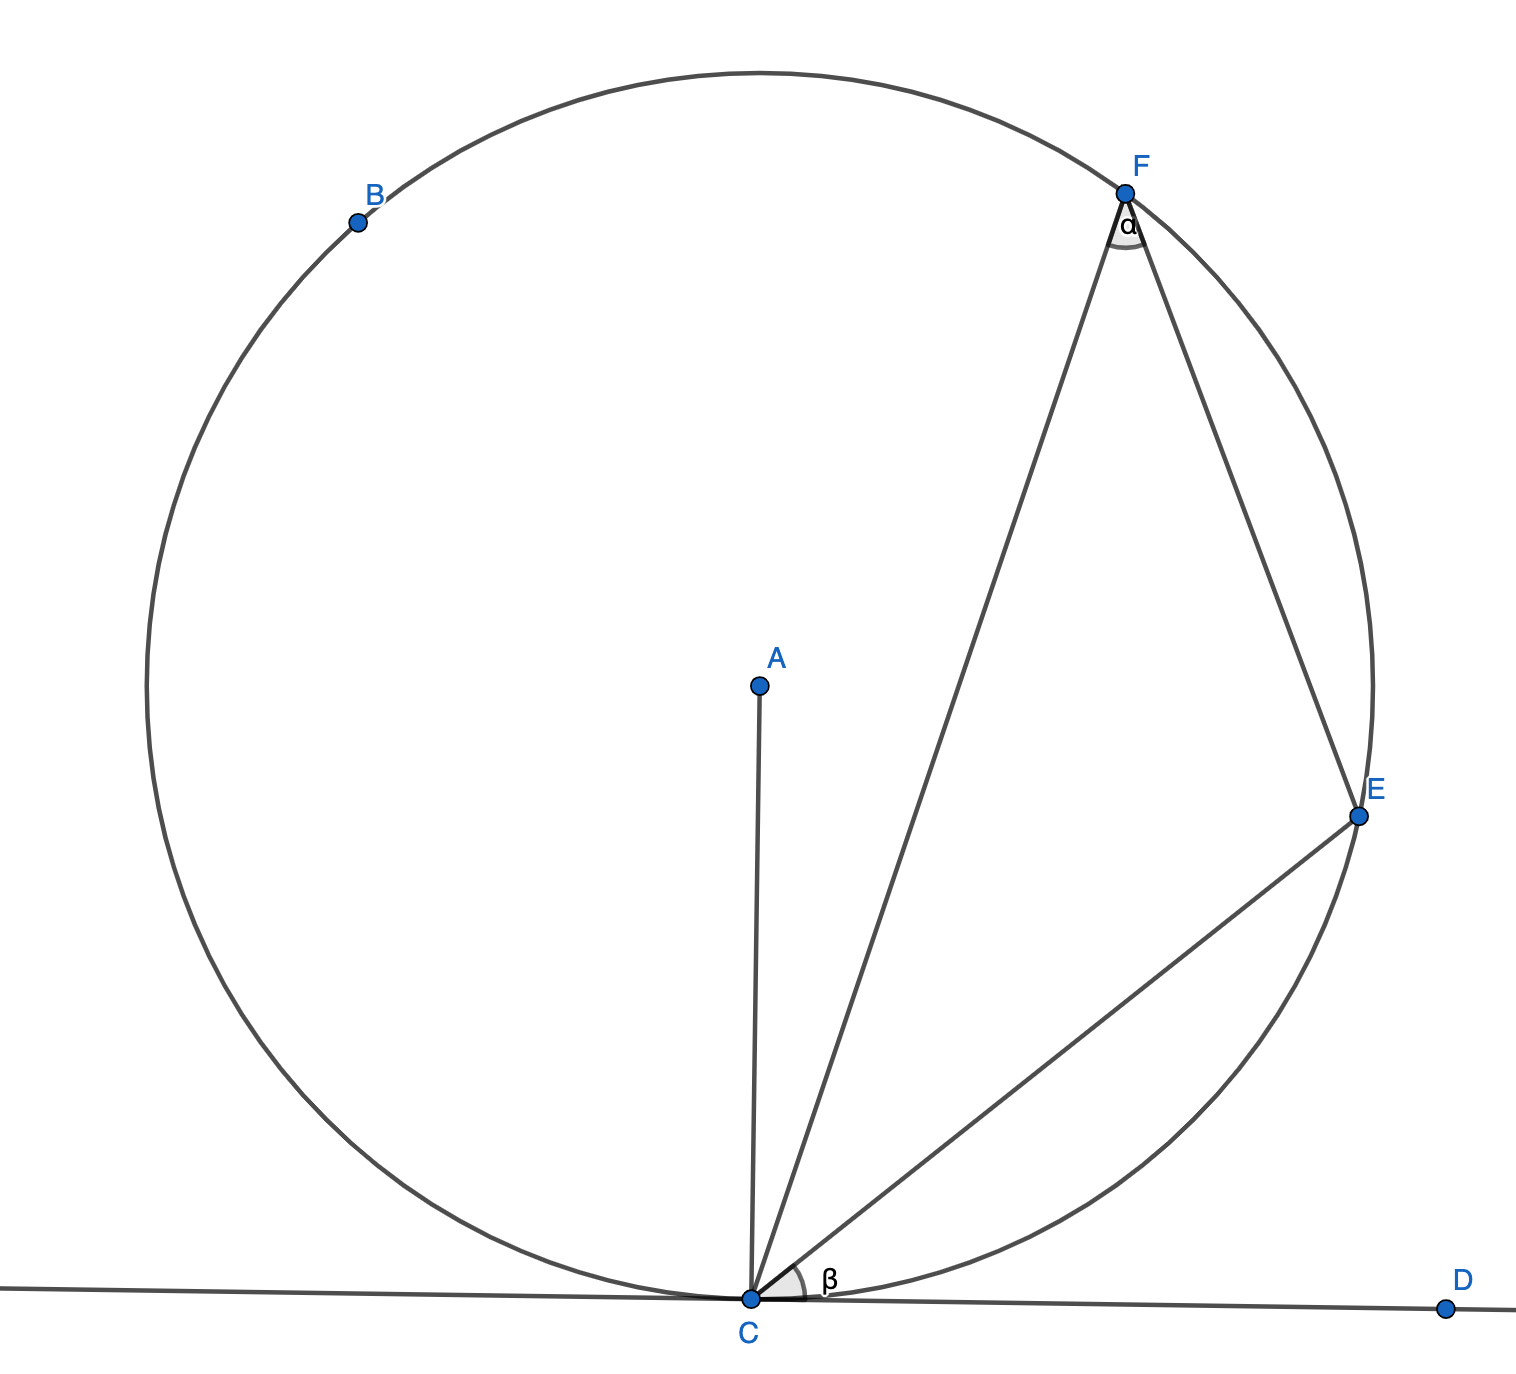
\includegraphics[width=\linewidth]{Chord_Tangent_Angle.png}
				\caption{Angle ECD is the chord tangent angle for chord $EC$ and tangent $CD$; angle PRQ is the inscribed angle of the arc CE;$\angle\ CDE=  \angle CDF$}
			\end{figure}
		\end{column}
		\begin{column}{0.6\textwidth} % Right column width

		\begin{theorem}[弦切角定理]
			The angle formed between a chord and a tangent line to a circle is equal to the inscribed angle on the other side of the chord.
		\end{theorem}
		\end{column}
	\end{columns}
\end{frame}

%------------------------------------------------



\begin{frame}
\frametitle{The Proof of Chord Tangent Angle Property}
\framesubtitle{弦切角定理证明}

\begin{columns}[t] 
		\begin{column}{0.4\textwidth} % Left column width
			\begin{figure}
				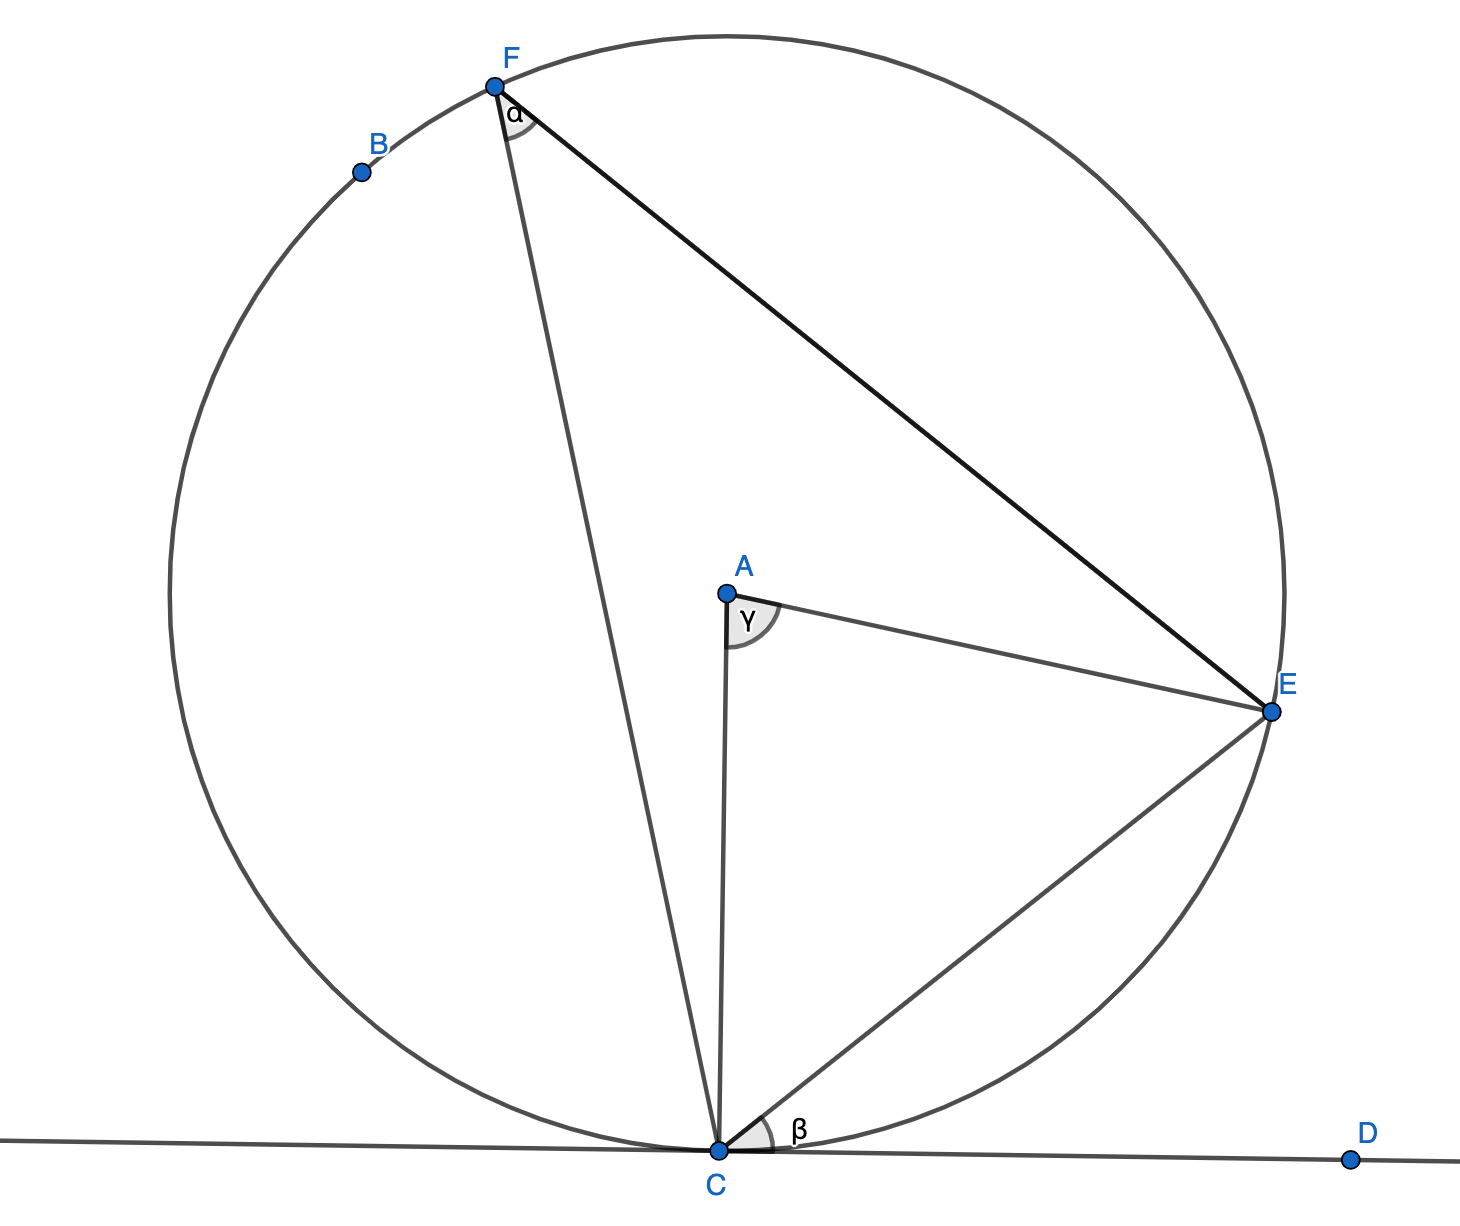
\includegraphics[width=\linewidth]{Chord_Tangent_Angle_Proof.png}
				\caption{$\angle\ CDE=  \angle CDF$}
			\end{figure}
		\end{column}
		\begin{column}{0.6\textwidth} % Right column width
			\begin{equation*}
			\begin{aligned}
			&\because AC = AE\\
			&\therefore\angle ACE = \angle AEC\\
			&\because \angle CAE = 2 \angle CFE\\
			&\therefore \angle CAE + \angle ACE + \angle AEC
			&= 2(\angle CFE  + \angle ACE)\\
			&= \ang{360}\\
			&\therefore \angle CFE  + \angle ACE = \ang{90}\\
			&\because \angle ECD  + \angle ACE = \ang{90}\\
			&\therefore \angle CFE = \angle ECD \ Q.E.D.
			\end{aligned}
			\end{equation*}		
		\end{column}
	\end{columns}
\end{frame}

%------------------------------------------------


\begin{frame}
	\frametitle{A Real QR Problem!}
	\framesubtitle{}
	\begin{figure}
		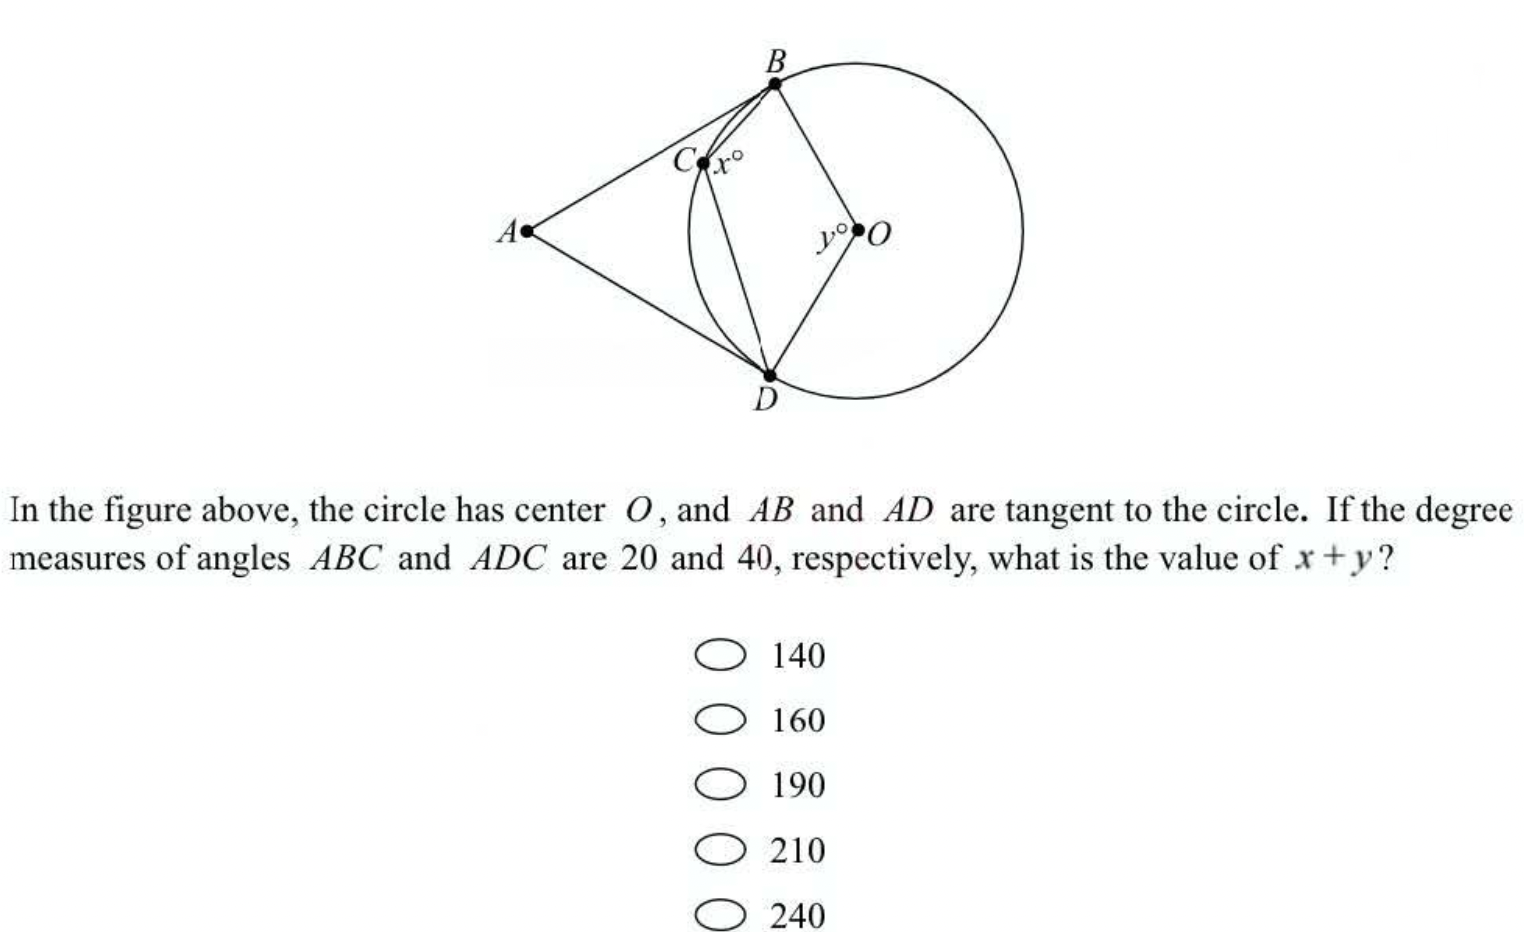
\includegraphics[width=0.8\linewidth]{Chord_Angle_Tangent_Example_Question1.png}
		\caption{10-Sec1-19}
	\end{figure}
\end{frame}

%------------------------------------------------

\begin{frame}
	\frametitle{Answer}
	\framesubtitle{Arc和Central Angle等比例}
	\pause
	\begin{columns}[t] 
		\begin{column}{0.4\textwidth} % Left column width
			\begin{figure}
				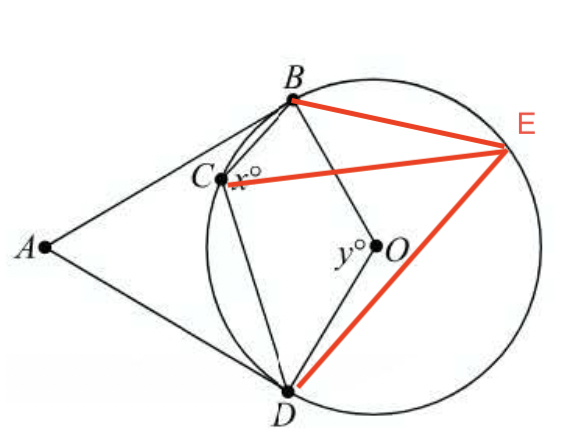
\includegraphics[width=\linewidth]{Chord_Angle_Tangent_Example_Question1_1.png}
			\end{figure}
			\pause
			Answer \textbf{E $240$}
		\end{column}
		\begin{column}{0.6\textwidth} % Right column width
			\pause
	     \begin{equation*}
					\begin{aligned}
					&\because \widearc{BC}\\
					&\therefore \angle BOC = 2 \angle ABC = \ang{40}\\
					&similarly, \\
					&\angle COD = 2 \angle CDA =\ang{80}\\
					& \therefore \widearc{BCD}\ has\ central \ angle \\
					&\angle BOD = \ang{120}\\
					&\therefore \widearc{BD}\ has\ central \ angle \\
					&\ang{360} - \angle BOD =\ang{240}\\
					&\therefore \angle BCD = \frac{1}{2} \ang{240}=\ang{120}\\
					&\therefore x + y = \ang{120} + \ang{120} = \ang{240} 
					\end{aligned}
				\end{equation*}	
		\end{column}
	\end{columns}
			
\end{frame}

%------------------------------------------------

\subsection{Inscribe v.s. Circumscribe}

%------------------------------------------------

\begin{frame}
\frametitle{Inscribed Polygon in a Circle}
\framesubtitle{外接圆}

\begin{columns}[t] 
		\begin{column}{0.4\textwidth} % Left column width
			\begin{figure}
				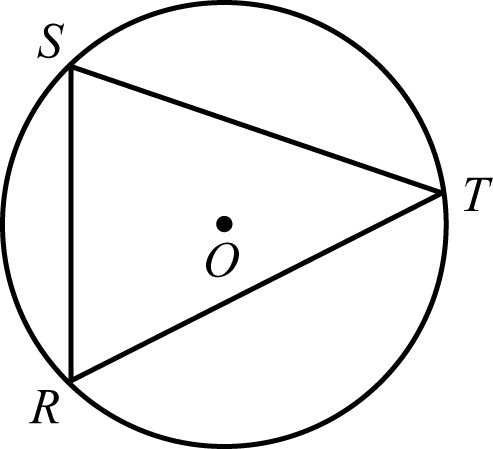
\includegraphics[width=\linewidth]{Inscribe.jpg}
				\caption{The vertices of triangle $STR$ are located on the circle $O$.}
			\end{figure}
		\end{column}
		\begin{column}{0.6\textwidth} % Right column width
		\begin{definition}
			A polygon is inscribed in a circle if all its vertices lie on the circle.
		\end{definition}
		\pause "the circle is circumscribed about the polygon." 谁在外面谁在里面? \pause \alert{\textbf{还是外接圆}}
		\end{column}
	\end{columns}
\end{frame}

%------------------------------------------------

\begin{frame}
	\frametitle{Math Vocab!} % Slide title, remove this command for no title
	\framesubtitle{专业名词记忆时间!}
	\begin{columns}[t] 
	\begin{column}{0.45\textwidth} % Left column width
		{\Huge inscribe}\\
		{\LARGE /inˈskrīb/\\
			\bigskip\bigskip
			draw (a figure) \alert{within} another so that their boundaries touch but do not intersect.
		A is inscribed in B: A被B外接, 在里面画}
	\end{column}
	\begin{column}{0.45\textwidth} % Right column width
		{\Huge circumscribe}\\
		{\LARGE /ˈsərkəmˌskrīb/\\
			\bigskip\bigskip
			draw (a figure) around another, touching it at points but not cutting it.
		A is circumscribed about B: A外接B,在外面画}	
	\end{column}
\end{columns}
\end{frame}

%------------------------------------------------

\begin{frame}
\frametitle{Thales's theorem}
\framesubtitle{如果三角形边长为外接圆直径,直径对角为直角}

\begin{columns}[t] 
		\begin{column}{0.4\textwidth} % Left column width
			\begin{figure}
				\includegraphics[width=\linewidth]{Inscribe_Right.jpg}
				\caption{$XZ$ is the diameter of the circle $W$; $\angle XYZ = \ang{90}	$}
			\end{figure}
		\end{column}
		\begin{column}{0.6\textwidth} % Right column width
		\begin{definition}
			if X, Z, and Y are distinct points on a circle where the line $XZ$ is a diameter, the angle $ABC$ is a right angle.
		\end{definition}
		\end{column}
	\end{columns}
\end{frame}

%------------------------------------------------


\begin{frame}
	\frametitle{A Real QR Problem!}
	\framesubtitle{自己画图!}
	\begin{figure}
		\includegraphics[width=\linewidth]{Inscribe_Example_Question1.png}
		\caption{7-Sec2-5}
	\end{figure}

\end{frame}

%------------------------------------------------


\begin{frame}
	\frametitle{Answer}
	\begin{columns}[t] 

		\begin{column}{0.5\textwidth} % Left column width
			\begin{figure}
				\includegraphics[width=\linewidth]{Inscribe_Example_Question1_1.png}
			\end{figure}
		\end{column}

		\begin{column}{0.5\textwidth} % Right column width
			\begin{equation*}
				\begin{aligned}
					&perimeter = \frac{\sqrt{2}}{2}d + \frac{\sqrt{2}}{2}d + d\\
					&=\sqrt{2}d + d \\
					&>\frac{5}{2}d
				\end{aligned}
			\end{equation*}	
		  Answer \textbf{B} Quantity B is greater
		\end{column}

	\end{columns}
\end{frame}

%------------------------------------------------

\begin{frame}
\frametitle{Circumscribed Polygon in a Circle}
\framesubtitle{内切圆}

\begin{columns}[t] 
		\begin{column}{0.4\textwidth} % Left column width
			\begin{figure}
				\includegraphics[width=\linewidth]{Circumscribed.jpg}
				\caption{quadrilateral $ABCD$ circumscribed about a circle with center $O$.}
			\end{figure}
		\end{column}
		\begin{column}{0.6\textwidth} % Right column width
		\begin{definition}
			A polygon is circumscribed about a circle if each side of the polygon is tangent to the circle, or equivalently, the circle is inscribed in the polygon.
		\end{definition}
		\end{column}
	\end{columns}
\end{frame}

%------------------------------------------------

\subsection{Concentric Circles}

%------------------------------------------------

\begin{frame}
\frametitle{Concentric Circles}
\framesubtitle{同心圆}

\begin{columns}[t] 
		\begin{column}{0.4\textwidth} % Left column width
			\begin{figure}
				\includegraphics[width=\linewidth]{Concentric.jpg}
			\end{figure}
		\end{column}
		\begin{column}{0.6\textwidth} % Right column width
		\begin{definition}
Two or more circles with the same center are called concentric circles.		
\end{definition}
\pause You must have known eccentric!
		\end{column}
	\end{columns}
\end{frame}

%------------------------------------------------

\section{Polygons}

%------------------------------------------------

\begin{frame}
	\frametitle{Math Vocab!} % Slide title, remove this command for no title
	\framesubtitle{专业名词记忆时间!}
	
	{\Huge polygons}\\
	{\LARGE /ˈpälēˌɡän/\
		\bigskip\bigskip
	a plane figure with at least three straight sides and angles, and typically five or more. \\ 
	多边形}

\end{frame}

%------------------------------------------------


\begin{frame}
	\frametitle{The Sum Of The Measures Of The Interior Angles} % Slide title, remove this command for no title
	\framesubtitle{多边形内角和}
	\begin{theorem}
		If a polygon has n sides, it can be divided into n − 2 triangles. Since the
sum of the measures of the interior angles of a triangle is 180°, it follows that
the sum of the measures of the interior angles of an n-sided polygon is $(n − 2)(\ang{180})$.
	\end{theorem}
	\begin{figure}
		\includegraphics[width=\linewidth]{Interior_Angles_Polygon.jpg}
		\caption{$(4-2)(\ang{180})=\ang{360}$(Left); $(5-2)(\ang{180})=\ang{540}$(Right)}
	\end{figure}
\end{frame}	

%------------------------------------------------

\begin{frame}
	\frametitle{Math Vocab!} % Slide title, remove this command for no title
	\framesubtitle{专业名词记忆时间!}
	
	{\Huge perimeter}\\
	{\LARGE /pəˈrimidər/\\
		\bigskip\bigskip
	the continuous line forming the boundary of a closed geometric figure. \\ 
	周长}

\end{frame}

%------------------------------------------------

\begin{frame}
	\frametitle{Regular Polygon} % Slide title, remove this command for no title
	\framesubtitle{正多边形}
	\begin{definition}
		A polygon in which all sides are congruent and all interior angles are
congruent is called a regular polygon.
	\end{definition}
	\begin{figure}
		\includegraphics[width=\linewidth]{Regular_Polygons.jpeg}
	\end{figure}
\end{frame}	

%------------------------------------------------


\begin{frame}
	\frametitle{Math Vocab!} % Slide title, remove this command for no title
	\framesubtitle{专业名词记忆时间!}
	

	\begin{columns}[t] 
	\begin{column}{0.4\textwidth} % Left column width
		{\Huge pentagon}\\
		{\LARGE /ˈpen(t)əˌɡän/\\
			\bigskip\bigskip
		五边形}
	\end{column}
	\begin{column}{0.6\textwidth} % Right column width
		\begin{figure}
			\includegraphics[width=0.8\linewidth]{220px-Regular_polygon_5_annotated.svg.png}
			\caption{The regular pentagon}
		\end{figure}	
	\end{column}
\end{columns}

\end{frame}

%------------------------------------------------



\begin{frame}
	\frametitle{Math Vocab!} % Slide title, remove this command for no title
	\framesubtitle{专业名词记忆时间!}
	

	\begin{columns}[t] 
	\begin{column}{0.4\textwidth} % Left column width
		{\Huge hexagon}\\
		{\LARGE /ˈheksəˌɡän/\\
			\bigskip\bigskip
		六边形}
	\end{column}
	\begin{column}{0.6\textwidth} % Right column width
		\begin{figure}
			\includegraphics[width=0.8\linewidth]{hexagon.png}
			\caption{The regular hexagon}
		\end{figure}	
	\end{column}
\end{columns}

\end{frame}

%------------------------------------------------


\begin{frame}
	\frametitle{A Real QR Problem!}
	\framesubtitle{注意看清楚题目要求!"Approximately!"}
	\begin{figure}
		\includegraphics[width=0.8\linewidth]{Hexagon_Triangle_Example_Question1.png}
		\caption{7-Sec2-13}
	\end{figure}
\end{frame}

%------------------------------------------------

\begin{frame}
	\frametitle{Answer}
	\framesubtitle{}
	\begin{columns}[t] 
		\begin{column}{0.3\textwidth} % Left column width
			\begin{figure}
				\includegraphics[width=\linewidth]{Hexagon_Triangle_Example_Question1_1.png}
			\end{figure}
			\pause
			Answer \textbf{B $9$}		
		\end{column}
		\begin{column}{0.7\textwidth} % Right column width
			\pause
	     \begin{equation*}
					\begin{aligned}
					r       &= 4\\
					S_{hex} &= 6 \cdot\frac{1}{2}\cdot r\cdot (\frac{\sqrt{3}}{2}r)\\
					        &= 6\cdot\frac{1}{2} \cdot4\cdot (\frac{\sqrt{3}}{2}4)\\
					        &= 6\cdot\frac{1}{2} \cdot4\cdot(\frac{\sqrt{3}}{2}4)\\
					        &= 24\sqrt{3}\\
					S_{cir} &= \pi r^2 = 16 \pi\\
					S_{shaded} &= S_{cir} - S_{hex}\\
					           &= 16 \pi -24\sqrt{3}\\
					           &\approx 8.67
					\end{aligned}
				\end{equation*}					
		\end{column}
	\end{columns}
\end{frame}

%------------------------------------------------



\begin{frame}
	\frametitle{Math Vocab!} % Slide title, remove this command for no title
	\framesubtitle{专业名词记忆时间!}
	
	\begin{columns}[t] 
	\begin{column}{0.4\textwidth} % Left column width
		{\Huge heptagon}\\
		{\LARGE /ˈheptəˌɡän/\\
			\bigskip\bigskip
		七边形}
	\end{column}
	\begin{column}{0.6\textwidth} % Right column width
		\begin{figure}
			\includegraphics[width=0.8\linewidth]{heptagon.png}
			\caption{The regular heptagon}
		\end{figure}	
	\end{column}
\end{columns}
\end{frame}

%------------------------------------------------


\begin{frame}
	\frametitle{Math Vocab!} % Slide title, remove this command for no title
	\framesubtitle{专业名词记忆时间!}
	
	\begin{columns}[t] 
	\begin{column}{0.4\textwidth} % Left column width
		{\Huge octagon}\\
		{\LARGE /ˈäktəˌɡän,ˈäktəˌɡən/\\
			\bigskip\bigskip
		八边形}
	\end{column}
	\begin{column}{0.6\textwidth} % Right column width
		\begin{figure}
			\includegraphics[width=0.8\linewidth]{octagon.png}
			\caption{The regular octagon}
		\end{figure}	
	\end{column}
\end{columns}
\end{frame}

%------------------------------------------------

\begin{frame}
	\frametitle{Math Vocab!} % Slide title, remove this command for no title
	\framesubtitle{专业名词记忆时间!}
	
	\begin{columns}[t] 
	\begin{column}{0.4\textwidth} % Left column width
		{\Huge nonagon}\\
		{\LARGE /ˈnänəˌɡän,ˈnōnəˌɡän/\\
			\bigskip\bigskip
		九边形}
	\end{column}
	\begin{column}{0.6\textwidth} % Right column width
		\begin{figure}
			\includegraphics[width=0.8\linewidth]{nonagon.png}
			\caption{The regular nonagon}
		\end{figure}	
	\end{column}
\end{columns}
\end{frame}

%------------------------------------------------

\begin{frame}
	\frametitle{Math Vocab!} % Slide title, remove this command for no title
	\framesubtitle{专业名词记忆时间!}
	
	\begin{columns}[t] 
	\begin{column}{0.4\textwidth} % Left column width
		{\Huge decagon}\\
		{\LARGE /ˈdekəˌɡän/\\
			\bigskip\bigskip
		十边形}
	\end{column}
	\begin{column}{0.6\textwidth} % Right column width
		\begin{figure}
			\includegraphics[width=0.8\linewidth]{decagon.png}
			\caption{The regular decagon}
		\end{figure}	
	\end{column}
\end{columns}
\end{frame}

%------------------------------------------------


\begin{frame}
	\frametitle{Mnemonic} % Slide title, remove this command for no title
	\framesubtitle{助记方法:结尾都是gon,开头是数字前缀}
	\begin{table}
		\begin{tabularx}{350pt}{c X X}
			\toprule
			\textbf{The Number Prefix} & \textbf{Derived Words} & \textbf{The Interior Angle $\frac{(n-2)\ang{360}}{n}$}\\
			\midrule
			penta- & 美国国防部五角大楼 & \ang{108}\\
			\midrule
			hexa- & hexacode六位数字表达颜色,蓝色\#0000FF & \ang{120}\\
			\midrule
			hepta- & semtemper 罗马日历的第7个月 & $128\frac{4}{7}$\textdegree\\
			\midrule
			octa- & octopus 八爪鱼 & \ang{135}\\
			\midrule
			nona- & November 罗马日历的第9个月 & \ang{140}\\
			\midrule
			deca- & decade 十年 & \ang{144}\\
			\bottomrule
		\end{tabularx}
	\end{table}
\end{frame}

%------------------------------------------------



\begin{frame}% The optional argument 'plain' hides the headline and footline
\frametitle{In-class Quiz}
\framesubtitle{写不出来的,可以写一个大概}
	\begin{center}
		{\Huge 1 Min}
		\bigskip\bigskip % Vertical whitespace
		
		{\LARGE State the name of polygons with 5 to 10 sides.}
	\end{center}
\end{frame}


%------------------------------------------------


\section{Three-Dimensional Figures}

%------------------------------------------------

\subsection{Rectangular Solid(Right Rectangular Prism)}

%------------------------------------------------

\begin{frame}
\frametitle{Rectangular Solid(Right Rectangular Prism)}
\framesubtitle{立方体(正四棱柱)}
	\begin{columns}[t] 
			\begin{column}{0.4\textwidth} % Left column width
			\begin{equation*}
			\begin{aligned}
			&Volume: \ V = lwh\\
			&Surface\ Area:\ A = 2(lw + lh + wh)
			\end{aligned}
			\end{equation*}	

			\end{column}
			\begin{column}{0.6\textwidth} % Right column width
				\begin{figure}
				\includegraphics[width=\linewidth]{Rectangular_Solid.jpg}
			\end{figure}
			\end{column}
		\end{columns}
\end{frame}

%------------------------------------------------



\begin{frame}
	\frametitle{A Real QR Problem!}
	\framesubtitle{可以不画图}
	\begin{figure}
		\includegraphics[width=\linewidth]{Rectangular_Solid_Example_Question1.png}
		\caption{4-Sec3-12}
	\end{figure}
\end{frame}

%------------------------------------------------

\begin{frame}
	\frametitle{Answer}
	\framesubtitle{}
	\pause
	\begin{columns}[t] 
		\begin{column}{0.6\textwidth} % Left column width
			\begin{figure}
				\includegraphics[width=\linewidth]{Rectangular_Solid_Example_Question1_1.png}
			\end{figure}
			\pause
			Answer \textbf{C $8.71$}
		\end{column}
		\begin{column}{0.4\textwidth} % Right column width
			\pause
	     \begin{equation*}
					\begin{aligned}
					&d = (1 - 0.2)c = 1.2c\\
					&a = (1-\frac{x}{100})b\\
					&a^2 d \\
					&=(1-\frac{x}{100})^2b^21.2c\\
					&= 1.2(1-\frac{x}{100})^2b^2c\\
					&=b^2c\\
					&\therefore1.2(1-\frac{x}{100})^2=1\\
					&x = (1 - \sqrt{\frac{5}{6}}) \cdot 100\\
					&\approx 8.71\\
					\end{aligned}
				\end{equation*}	
		\end{column}
	\end{columns}
\end{frame}

%------------------------------------------------

\subsection{Circular Cylinder And Right Circular Cylinder}

%------------------------------------------------

\begin{frame}
\frametitle{ Right Circular Cylinder}
\framesubtitle{正圆柱}

\begin{columns}[t] 
		\begin{column}{0.6\textwidth} % Left column width
			\begin{equation*}
			\begin{aligned}
			&Volume: \ V = \pi r^2h\\
			&Surface\ Area:\ A = 2\pi r^2 + 2\pi r h
			\end{aligned}
			\end{equation*}		

		\end{column}
		\begin{column}{0.2\textwidth} % Right column width
			\begin{figure}
				\includegraphics[width=\linewidth]{Right_Circular_Cylinder.jpg}
			\end{figure}
		\end{column}
	\end{columns}
\end{frame}

%------------------------------------------------
% 	\begin{columns}[t] 
% 		\begin{column}{0.5\textwidth} % Left column width
% 		\end{column}
% 		\begin{column}{0.5\textwidth} % Right column width
% 		\end{column}
% 	\end{columns}


% 	\begin{figure}
% 		\includegraphics[width=0.8\linewidth]{creodocs_logo.pdf}
% 		\caption{Creodocs logo.}
% 	\end{figure}


% \begin{frame}
% 	\frametitle{A Real QR Problem!}
% 	\framesubtitle{}
% 	\begin{figure}
% 		\includegraphics[width=\linewidth]{Percent_Increase_Example_Question1.png}
% 		\caption{-Sec-}
% 	\end{figure}
% 	\pause
% $$ \\
% \pause
% \bigskip
% Answer \textbf{B } 
% \end{frame}

% %------------------------------------------------


%------------------------------------------------

% \begin{frame}
% 	\frametitle{Have a try!}
% 	\framesubtitle{}


% \bigskip
% \pause

% \bigskip
% Answer \textbf{- 2.48\%}
% \end{frame}

% %------------------------------------------------
%------------------------------------------------
% \section{Text Examples} % Sections are added in order to organize your presentation into discrete blocks, all sections and subsections are automatically output to the table of contents as an overview of the talk but NOT output in the presentation as separate slides

% %------------------------------------------------

% \subsection{Paragraphs and Lists}

% \begin{frame}
% 	\frametitle{Paragraphs of Text}
	
% 	Sed iaculis \alert{dapibus gravida}. Morbi sed tortor erat, nec interdum arcu. Sed id lorem lectus. Quisque viverra augue id sem ornare non aliquam nibh tristique. Aenean in ligula nisl. Nulla sed tellus ipsum. Donec vestibulum ligula non lorem vulputate fermentum accumsan neque mollis.
	
% 	\bigskip % Vertical whitespace
	
% 	% Quote example
% 	\begin{quote}
% 		Sed diam enim, sagittis nec condimentum sit amet, ullamcorper sit amet libero. Aliquam vel dui orci, a porta odio.\\
% 		--- Someone, somewhere\ldots
% 	\end{quote}
	
% 	\bigskip % Vertical whitespace
	
% 	Nullam id suscipit ipsum. Aenean lobortis commodo sem, ut commodo leo gravida vitae. Pellentesque vehicula ante iaculis arcu pretium rutrum eget sit amet purus. Integer ornare nulla quis neque ultrices lobortis.
% \end{frame}

% %------------------------------------------------

% \begin{frame}
% 	\frametitle{Lists}
% 	\framesubtitle{Bullet Points and Numbered Lists} % Optional subtitle
	
% 	\begin{itemize}
% 		\item Lorem ipsum dolor sit amet, consectetur adipiscing elit
% 		\item Aliquam blandit faucibus nisi, sit amet dapibus enim tempus
% 		\begin{itemize}
% 			\item Lorem ipsum dolor sit amet, consectetur adipiscing elit
% 			\item Nam cursus est eget velit posuere pellentesque
% 		\end{itemize}
% 		\item Nulla commodo, erat quis gravida posuere, elit lacus lobortis est, quis porttitor odio mauris at libero
% 	\end{itemize}
	
% 	\bigskip % Vertical whitespace
	
% 	\begin{enumerate}
% 		\item Nam cursus est eget velit posuere pellentesque
% 		\item Vestibulum faucibus velit a augue condimentum quis convallis nulla gravida 
% 	\end{enumerate}
% \end{frame}

% %------------------------------------------------

% \subsection{Blocks}

% \begin{frame}
% 	\frametitle{Blocks of Highlighted Text}
	
% 	\begin{block}{Block Title}
% 		Lorem ipsum dolor sit amet, consectetur adipiscing elit. Integer lectus nisl, ultricies in feugiat rutrum, porttitor sit amet augue.
% 	\end{block}
	
% 	\begin{exampleblock}{Example Block Title}
% 		Aliquam ut tortor mauris. Sed volutpat ante purus, quis accumsan.
% 	\end{exampleblock}
	
% 	\begin{alertblock}{Alert Block Title}
% 		Pellentesque sed tellus purus. Class aptent taciti sociosqu ad litora torquent per conubia nostra, per inceptos himenaeos.
% 	\end{alertblock}
	
% 	\begin{block}{} % Block without title
% 		Suspendisse tincidunt sagittis gravida. Curabitur condimentum, enim sed venenatis rutrum, ipsum neque consectetur orci.
% 	\end{block}
% \end{frame}

% %------------------------------------------------

% \subsection{Columns}

% \begin{frame}
% 	\frametitle{Multiple Columns}
% 	\framesubtitle{Subtitle} % Optional subtitle
	
% 	\begin{columns}[t] 
% 		\begin{column}{0.5\textwidth} % Left column width
% 		\end{column}
% 		\begin{column}{0.5\textwidth} % Right column width
% 	\end{columns}





% \end{frame}

% %------------------------------------------------

% \section{Table and Figure Examples}

% \subsection{Table}

% \begin{frame}
% 	\frametitle{Table}
% 	\framesubtitle{Subtitle} % Optional subtitle
	
% 	\begin{table}
% 		\begin{tabular}{l l l}
% 			\toprule
% 			\textbf{Treatments} & \textbf{Response 1} & \textbf{Response 2}\\
% 			\midrule
% 			Treatment 1 & 0.0003262 & 0.562 \\
% 			Treatment 2 & 0.0015681 & 0.910 \\
% 			Treatment 3 & 0.0009271 & 0.296 \\
% 			\bottomrule
% 		\end{tabular}
% 		\caption{Table caption}
% 	\end{table}
% \end{frame}

% %------------------------------------------------

% \subsection{Figure}

% \begin{frame}
% 	\frametitle{Figure}
	
% 	\begin{figure}
% 		\includegraphics[width=0.8\linewidth]{creodocs_logo.pdf}
% 		\caption{Creodocs logo.}
% 	\end{figure}





% \end{frame}

% %------------------------------------------------

% \section{Mathematics}

% \begin{frame}
% 	\frametitle{Definitions \& Examples}
	
% 	\begin{definition}
% 		A \alert{prime number} is a number that has exactly two divisors.
% 	\end{definition}
	
% 	\smallskip % Vertical whitespace
	
% 	\begin{example}
% 		\begin{itemize}
% 			\item 2 is prime (two divisors: 1 and 2).
% 			\item 3 is prime (two divisors: 1 and 3).
% 			\item 4 is not prime (\alert{three} divisors: 1, 2, and 4).
% 		\end{itemize}
% 	\end{example}
	
% 	\smallskip % Vertical whitespace
	
% 	You can also use the \texttt{theorem}, \texttt{lemma}, \texttt{proof} and \texttt{corollary} environments.
% \end{frame}

% %------------------------------------------------

% \begin{frame}
% 	\frametitle{Theorem, Corollary \& Proof}
	
% 	\begin{theorem}[Mass--energy equivalence]
% 		$E = mc^2$
% 	\end{theorem}
	
% 	\begin{corollary}
% 		$x + y = y + x$
% 	\end{corollary}
	
% 	\begin{proof}
% 		$\omega + \phi = \epsilon$
% 	\end{proof}
% \end{frame}

% %------------------------------------------------

% \begin{frame}
% 	\frametitle{Equation}

% 	\begin{equation}
% 		\cos^3 \theta =\frac{1}{4}\cos\theta+\frac{3}{4}\cos 3\theta
% 	\end{equation}
% \end{frame}

% %------------------------------------------------

% \begin{frame}[fragile] % Need to use the fragile option when verbatim is used in the slide
% 	\frametitle{Verbatim}
	
% 	\begin{example}[Theorem Slide Code]
% 		\begin{verbatim}
% 			\begin{frame}
% 				\frametitle{Theorem}
% 				\begin{theorem}[Mass--energy equivalence]
% 					$E = mc^2$
% 				\end{theorem}
% 		\end{frame}\end{verbatim} % Must be on the same line
% 	\end{example}
% \end{frame}

% %------------------------------------------------

% \begin{frame}
% 	Slide without title.
% \end{frame}

% %------------------------------------------------

% \section{Referencing}

% \begin{frame}
% 	\frametitle{Citing References}
	
% 	An example of the \texttt{\textbackslash cite} command to cite within the presentation:
	
% 	\bigskip % Vertical whitespace
	
% 	This statement requires citation \cite{p1,p2}.
% \end{frame}

% %------------------------------------------------

% \begin{frame} % Use [allowframebreaks] to allow automatic splitting across slides if the content is too long
% 	\frametitle{References}
	
% 	\begin{thebibliography}{99} % Beamer does not support BibTeX so references must be inserted manually as below, you may need to use multiple columns and/or reduce the font size further if you have many references
% 		\footnotesize % Reduce the font size in the bibliography
		
% 		\bibitem[Smith, 2022]{p1}
% 			John Smith (2022)
% 			\newblock Publication title
% 			\newblock \emph{Journal Name} 12(3), 45 -- 678.
			
% 		\bibitem[Kennedy, 2023]{p2}
% 			Annabelle Kennedy (2023)
% 			\newblock Publication title
% 			\newblock \emph{Journal Name} 12(3), 45 -- 678.
% 	\end{thebibliography}
% \end{frame}

% %----------------------------------------------------------------------------------------
% %	ACKNOWLEDGMENTS SLIDE
% %----------------------------------------------------------------------------------------

% \begin{frame}
% 	\frametitle{Acknowledgements}
	
% 	\begin{columns}[t] % The "c" option specifies centered vertical alignment while the "t" option is used for top vertical alignment
% 		\begin{column}{0.45\textwidth} % Left column width
% 			\textbf{Smith Lab}
% 			\begin{itemize}
% 				\item Alice Smith
% 				\item Devon Brown
% 			\end{itemize}
% 			\textbf{Cook Lab}
% 			\begin{itemize}
% 				\item Margaret
% 				\item Jennifer
% 				\item Yuan
% 			\end{itemize}
% 		\end{column}		
% 		\begin{column}{0.5\textwidth} % Right column width
% 			\textbf{Funding}
% 			\begin{itemize}
% 				\item British Royal Navy
% 				\item Norwegian Government
% 			\end{itemize}
% 		\end{column}
% 	\end{columns}
% \end{frame}

%----------------------------------------------------------------------------------------
%	CLOSING SLIDE
%----------------------------------------------------------------------------------------

\begin{frame}[plain] % The optional argument 'plain' hides the headline and footline
	\begin{center}
		{\Huge 1 Min Break}
		\bigskip\bigskip % Vertical whitespace
		
		{\LARGE Questions? Comments?}
	\end{center}
\end{frame}

%----------------------------------------------------------------------------------------

\end{document} 